\documentclass[a4paper]{book}

% Standard preamble for WRAMP documentation
% Includes necessary packages, additional styles, and such.
\usepackage{wramp}

\title{COMP201 Reference}
\author{...}
\begin{document}

%\includegraphics{coverpage.ps}
%\newpage

\begin{Huge}
\vspace{2cm}
\textbf{Preface}\\
\vspace{1.5cm}
\end{Huge}

This manual is intended as an introduction to the use of the Basys3 FPGA when
programmed with a WRAMP processor.
This includes programming for WRAMP and using the physical capabilities of the boards.
It covers the basics of the WRAMP assembly language, the WRAMP tools, and the I/O
devices implemented on the Basys boards.

Although every effort has been made to make this manual accurate, it is
possible that there may be errors in it. If you find any, please report
them to the author.

This manual is an update to the one detailing the WRAMP architecture as
implemented on the original REX boards used by the University of Waikato.
It was mainly the product of a lot of hard work by Matt Jervis
and Jamie Curtis. Other people that contributed to its content
were Murray Pearson, Tony McGregor, and Dean Armstrong.
The update was written by Daniel Oosterwijk and Tyler Marriner in
tandem with their development of the Basys implementation of WRAMP.

This version was last updated on \today.


%\maketitle

Copyright (C) 2019 The University of Waikato, Hamilton, New Zealand.
Permission is granted to copy, distribute and/or modify this document
under the terms of the GNU Free Documentation License, Version 1.3
or any later version published by the Free Software Foundation;
with no Invariant Sections, no Front-Cover Texts, and no Back-Cover Texts.
A copy of the license is included in the section entitled "GNU
Free Documentation License".

\tableofcontents

\chapter{Introduction}
\label{chapter:intro}
\documentclass[a4paper,10pt]{article}
\setlength{\parindent}{0ex}
\setlength{\parskip}{1.5ex}
\usepackage[dvips]{graphicx}
\usepackage{epsfig}
\usepackage[a4paper, hmargin=25mm, vmargin=30mm, nohead]{geometry}

\usepackage{fancyhdr}
\fancypagestyle{rcsfooters}{
\fancyfoot[L]{\small $ $RCSfile: intro.tex,v $ $}
\fancyfoot[R]{\small $ $Revision: 1.3 $ $}
}

\renewcommand{\headrulewidth}{0pt}

%INCLUDE OUR GLOBALS
\usepackage{rex201}
\usepackage{styles201}
\usepackage{ex201}


\begin{document}

\EXHEADING{\INTRONO}{\INTROTITLE}{%
Verification Date:~\INTRODUE\\
Excercise Test Date:~\CWRAMPTESTDATE\\
}


\section{Assessment}
To show that you have completed this exercise to a satisfactory
standard you will be required to demonstrate at a verification session
that the program you wrote in \textbf{Question~\ref{ques:final}} 
of this exercise
runs correctly. In addition the marker may ask one or two questions so
they establish that you understand what you have done.  These
verification sessions will be held in Lab 1 during the following two
times:

\begin{itemize}
\item \INTRODUE~\MORNINGASSESS
\item \INTRODUE~\AFTERNOONASSESS 
\end{itemize}

In an attempt to ensure that the verification process runs smoothly
six machines in \ASSESSROOM\ will be booked for this purpose during the two
sessions. When it is your turn to have your program verified you
should log onto one of these machines and get your program ready to
run on the REX board. A marker will then verify your program. Once
your program has been verified you should log off immediately to allow
the next person to prepare to have their program verified.

In addition to the test there will be a closed book excercise test on
\textbf{\CWRAMPTEST}.  The test will cover material 
from excercises 2, 3 and 4.

The tutorial times are listed on the course webpage:

\begin{center}
\src{\WEBPAGEBASE}
\end{center}

\section{Ojectives}
The objective of this exercise is to familiarise 
yourself with writing, assembling, linking, running, and
debugging assembly code for the WRAMP processor and the REX board.

Before attempting this excercise you should have read the 
chapter `Introduction to Rex and WRAMP' in your course manual.  The material covered in this chapter of the manual \textbf{is examinable}.

\section{Questions}
\begin{enumerate}
\item\label{ques:first} Write a program which continually (i.e. is in
an infinite loop) reads the values on the switches and outputs the
value read to the two seven segment displays.  For example if the
switches are set to the pattern shown in Figure \ref{fig:switches} the
two seven segment displays should show \src{92}.

\item\label{ques:two} Modify your program in Question \ref{ques:first}
to continually output the number of switches currently set (in the
down position or one) to the seven segment display. For example if the
switches are set to the pattern shown in Figure \ref{fig:switches}
then the seven segment display should display \src{03}.

\item\label{ques:final} Modify the program written in Question
\ref{ques:two} to encrypt the count of set switches before outputting
it to the seven-segment display. The encryption algorithm to be
applied is the very simple mapping function defined in Table
\ref{table:encode}. For example, the value \src{4} encrypted would be
displayed as \src{05}, and the value \src{8} encrypted would be
displayed as \src{07}.
\end{enumerate}

\begin{figure}[!hb]
\begin{center}
%\begin{tabular}{|c|}
%\hline
\includegraphics[width=15cm]{switches.eps}
%\\
%\hline
%\end{tabular}
\caption{Example}
\label{fig:switches}
\end{center}
\end{figure}


\begin{table}
\begin{center}
\begin{tabular}{|c|c|}
\hline
\verb|       |0\verb|       | & \verb|       |1\verb|       | \\ \hline
1 & 0 \\ \hline
2 & 8 \\ \hline
3 & 2 \\ \hline
4 & 5 \\ \hline
5 & 4 \\ \hline
6 & 9 \\ \hline
7 & 3 \\ \hline
8 & 7 \\ 
\hline
\end{tabular}
\end{center}
\label{table:encode}
\caption{Mapping Function for Encryption Process}
\end{table}






\thispagestyle{rcsfooters}
\pagestyle{rcsfooters}
\end{document}
\chapter{Stack Guide}
\label{chapter:stack}
%%
%
% Body
%
%%
\section{WRAMP Stack Frame}

A stack is a term used to describe a `first in, last out' buffer. New
items are placed on the top of the stack, and must be removed before
older items. Two terms are commonly used to refer to the operations of
adding to, and removing values from a stack. A push operation puts a
new value at the very top of the stack, and a pop operation removes the
item from the top of the stack. These are the only operations allowed to
be performed on a stack, and there is no way to remove an older item
before a newer one. Stacks provide an ideal mechanism for passing
parameters to a function and providing storage for local variables and
temporary results inside a function. This document describes the
reasons a stack is used on the WRAMP architecture, how the stack is
created, and the conventions surrounding its use.

The WRAMP processor itself does not directly support a stack, but
it is possible to setup a stack in software. To achieve this, a block
of memory for the stack to reside in must be set aside. On the Basys
board, \WRAMPmon\ does this for you. The stack starts at the top of
memory, with new items placed at lower memory addresses. Because of
this, stacks on the WRAMP architecture are often referred to as
growing downwards.

%%%
%
% PUSH FIGURE
%
%%%
\begin{figure}[!hb]
\begin{center}
\begin{footnotesize}
\begin{tabular}{|c|c|c|}

\hline
%% Text....
\begin{minipage}[l]{7cm}
\vspace{\topsep}
\begin{verbatim}

push:
      # move the stack pointer down
      # by one to create space for 
      # a value to be pushed onto 
      # the stack.

      subui $sp, $sp, 1

      # store the contents of $2 onto
      # the new space on the stack

      sw $2, 0($sp)

\end{verbatim}
\end{minipage}
&
%% Fig before
\begin{minipage}[c]{3.5cm}
\begin{center}
\includegraphics[width=2.2cm]{stack_fig1_a.pdf}
%\vspace{0.1cm}

\emph{before}\\
\end{center}
\end{minipage}

&
%% Fig after
\begin{minipage}[c]{3.5cm}
\begin{center}
\includegraphics[width=2.2cm]{stack_fig1_b.pdf}


\emph{after}\\
\end{center}
\end{minipage}
\\
\hline
\end{tabular}
\begin{center}
\small{
\textbf{(a) WRAMP code}
\hspace{3.5cm}
\textbf{(b) Stack Diagrams}
}
\end{center}

\caption{Push}
\label{fig:stack_push}
\end{footnotesize}
\end{center}
\end{figure}
%%%
%
% End of PUSH figure
%
%%%

To place new items onto and remove existing items from the stack you
need a way to know the current address of the top of the stack. To
allow this, a register is set aside to store this address. This
register is referred to as the ``top of stack'' pointer, or more often
just the ``stack pointer''. By WRAMP convention, the stack pointer is stored
in register 14 and is referred to as \src{\$sp} in WRAMP assembly code.
Figure \ref{fig:stack_push}(a) shows example WRAMP code to ``push'' a new
value onto the stack and (b) shows the stack before and after the push operation. Figure \ref{fig:stack_pop} shows the WRAMP code and stack diagrams for a pop
operation.

%%%
%
% POP FIGURE
%
%%%
\begin{figure}[!ht]
\begin{center}
\begin{footnotesize}
\begin{tabular}{|c|c|c|}

\hline
%% Text....
\begin{minipage}[l]{7cm}
\vspace{\topsep}
\begin{verbatim}

pop:
      # pop into register 3 the value
      # stored on the top of the
      # stack

      lw $3, 0($sp)

      # Move the stack pointer up
      # by one to remove item

      addui $sp, $sp, 1

\end{verbatim}
\end{minipage}
&
%% Fig before
\begin{minipage}[c]{3.5cm}
\begin{center}
\includegraphics[width=2.2cm]{stack_fig2_a.pdf}
%\vspace{0.3cm}

\emph{before}\\
\end{center}
\end{minipage}

&
%% Fig after
\begin{minipage}[c]{3.5cm}
\begin{center}
\includegraphics[width=2.2cm]{stack_fig2_b.pdf}

%\vspace{0.3cm}
\emph{after}\\
\end{center}
\end{minipage}
\\
\hline
\end{tabular}
\begin{center}
\small{
\textbf{(a) WRAMP code}
\hspace{3.5cm}
\textbf{(b) Stack Diagrams}
}
\end{center}

\caption{Pop}
\label{fig:stack_pop}
\end{footnotesize}
\end{center}
\end{figure}
%%%
%
% End of POP figure
%
%%%
\vspace{0.2cm} %Push to the next page

\section{WRAMP Stack Conventions}
On the WRAMP architecture the stack is used to:

\begin{itemize}
\item store local variables that are not stored in registers
\item temporarily store the contents of registers so that a subroutine can use them while making sure the previous contents are preserved.
\item pass parameters to a subroutine
\end{itemize}

%%%
%
% Figure 3
%
%%%
\begin{figure}[!hbt]
\begin{footnotesize}
\begin{center}
\begin{tabular}{|p{10cm}|}
\hline
\begin{verbatim}
parent:
       addi $3, $0, 5
loop:
       beqz $3, endloop
        ...
       jal child
        ...
       subi $3, $3, 1
       j loop

endloop:
       j exit

child:
        ...
       add $3, $4, $5
        ...
       jr $ra
\end{verbatim}
\\
\hline
\end{tabular}
\end{center}
\end{footnotesize}
\caption{Incorrect Function} 
\label{fig:problemcode}
\end{figure}

\section{Saving Registers}
When a program contains a number of subroutines that can call each
other, a set of conventions is required to ensure that a subroutine
does not use a register and modify values that a parent subroutine is
also using. For example consider the code sequence in Figure
\ref{fig:problemcode}. Notice that the section of code labelled
\src{parent} is using \src{\$3} as a loop counter that decrements each
time through the loop. Inside this loop is a call to the subroutine
\src{child} that uses \src{\$3} to store an intermediate result. This
would overwrite the loop counter value stored in that register by the
subroutine \src{parent}. While it would be possible in this simple
sequence to rearrange the code to fix the problem, it will not always
be possible to do so. To ensure problems like this do not occur in
code there needs to be a set of conventions controlling the way
registers are used.

The convention used in the WRAMP architecture is that all subroutines
must save the contents of a register to the stack before it can use
it. The value must then be restored from the stack before the
subroutine exits. It should be noted that it is up to the programmer
to ensure these conventions are followed and the processor does not
enforce them in any way. For code generated by a C compiler, the
compiler must ensure that these same conventions are followed. Figure
\ref{fig:correctcode} shows the corrected program that follows the
conventions.

When a subroutine is called using the \src{jal} instruction, the
return address for the subroutine is placed in register 15
(\src{\$ra}). If this subroutine then uses \src{jal} to call another
subroutine it will overwrite its own return address. Because of this,
any subroutine that is going to call another subroutine needs to save
\src{\$ra} onto the stack before calling the routine and restore it
before it returns. Figure \ref{savera} gives an example of this.


%%
%
% Figure 4
%
%%%
\begin{figure}[!hb]
\begin{footnotesize}
\begin{center}
\begin{tabular}{|p{10cm}|}
\hline
\begin{verbatim}
parent:
       addi  $3, $0, 5
loop:
       beqz  $3, endloop
        ...
       jal   child
        ...
       subi  $3, $3, 1
       j     loop

endloop:
       j exit

child:
        ...
       # save register 3 before we overwrite
       # the contents of it
       subui $sp, $sp, 1
       sw    $3, 0($sp)

       add   $3, $4, $5
        ...
       # restore the old contents of register
       # 3 before we return
       lw    $3, 0($sp)
       addui $sp, $sp, 1

       jr    $ra
\end{verbatim}
\\
\hline
\end{tabular}
\end{center}
\end{footnotesize}
\caption{Correct Function}
\label{fig:correctcode}
\end{figure}

There is one exception to the rule that all registers must be
saved. For reasons discussed in the next section, register 1
(\src{\$1}) never needs to be saved or restored.

\section{Parameter Passing}
In Chapter \ref{chapter:intro}, parameters were passed to
subroutines using regsiters. While this works in this simple case
consider what would happen if a subroutine required a large number of
parameters or called other subroutines. It is not difficult to see that
with a large program it would not take long to exhaust the registers
available to the programmer on the WRAMP processor.

%%%
%
% Figure 5
%
%%%
\begin{figure}[!htbp]
\begin{footnotesize}
\begin{center}
\begin{tabular}{|p{10cm}|}
\hline
\begin{verbatim}
child:
       # save the return address before we
       # call our subroutine
       subui $sp, $sp, 1
       sw $ra, 0($sp)

       jal my_child
        ...

       # get our return address back off of the
       # stack so we can return there.
       lw $ra, 0($sp)
       addui $sp, $sp, 1

       jr $ra
\end{verbatim}
\\
\hline
\end{tabular}
\end{center}
\end{footnotesize}
\caption{Calling a Function}
\label{savera}
\end{figure}

A convention needs to be defined so that a subroutine knows how to
find the parameters it has been passed, and knows how to pass
parameters to subroutines it calls.

On the WRAMP processor the convention is to pass all parameters to a
subroutine using the stack. Before a subroutine is called all of the
parameters that are going to be passed to it must first be pushed onto
the stack. Parameters appear on the very top of the stack when a
subroutine is entered. If code is being generated for a C function
call, then the convention is to push the parameters onto the stack in
the reverse order so that the first C parameter ends up on the top of
the stack just before the function is called. Figure
\ref{fig:parampassing}(a) shows a C function call, (b) WRAMP code to
implement it and (c) a diagram of the stack at the time of the
function call.

%%%
%
% Fig6: Param Passing
%
%%%
\begin{figure}[!hbtp]
\begin{center}
\begin{footnotesize}
\begin{tabular}{|c|c|c|}
\hline
\begin{minipage}[t]{4.8cm}
\begin{verbatim}

cat(first, second, third);

\end{verbatim}
%$
\end{minipage}
&
\begin{minipage}[c]{5.5cm}
\vspace{\topsep}
\begin{verbatim}

# push the third parameter on
subui $sp, $sp, 1
sw $3, 0($sp)

# push the second parameter on
subui $sp, $sp, 1
sw $4, 0($sp)

# push the first parameter on
subui $sp, $sp, 1
sw $5, 0($sp)

jal cat

# remove all three parameters
addui $sp, $sp, 3

\end{verbatim}
%$
\end{minipage}
&
\begin{minipage}{4.2cm}
\begin{center}
\includegraphics[width=3cm]{stack_fig6_a.pdf}
\end{center}
\end{minipage}\\
\hline
\end{tabular}
\\
\textbf{(a) C code}
\hspace{3cm}
\textbf{(b) WRAMP code}
\hspace{3cm}
\textbf{(c) Stack before call}\\

\caption{Passing Parameters to a Function}
\label{fig:parampassing}
\end{footnotesize}
\end{center}
\end{figure}

As you will notice in the previous example, a significant proportion of
the WRAMP code is associated with manipulating the stack pointer. An
alternative and more efficient approach is to calculate the maximum
size that a stack will grow to in a function and pre-allocate this
space as the function is entered. Just before this "parent" function
calls another function it copies the parameters to the appropriate
place in the pre-allocated space. If the function accepts one
parameter, that parameter must be placed at the top of the stack. If a
function accepts two parameters the first parameter must be placed at
the top of the stack and the second placed beneath it. If you think
of the parameters as a list numbered from zero, the position of any
parameter can be calculated as follows:

\begin{center}
$Address = \$sp + ParameterNumber$\\
\end{center}

For example if a function \src{cat(first, second, third)} is going to
be called then first will be placed at \mbox{\src{\$sp} + 0}, second
at \mbox{\src{\$sp} + 1} and third at \mbox{\src{\$sp} + 2}. Figure
\ref{fig:paramcalling}(a) shows an example C code sequence containing two
function calls (one with a single parameter and one with three
parameters) and Figure \ref{fig:paramcalling}(b) shows the WRAMP
assembly code for this sequence.

Once a subroutine has been called it then has to retrieve these
parameters off of the stack so that it can use them. This requires a
number of loads from the current stack. The important part to notice
is that these are not pop operations, as they do not reduce the size
of the stack. The function is simply looking into the stack of the
function that called it to discover the parameters it has been called
with. A function must \textbf{\emph{never}} return with the stack
pointer pointing to a different location than when the function was
called.

A function also needs to be able to return a value to its
parent. Traditional languages only ever allow a function to return a
single value, therefore the use of the stack to return a value is
probably over complex. On the WRAMP architecture, values are returned
to the parent in register 1 (\src{\$1}). Because of this fact,
\src{\$1} is the only exception to the rule that all registers must be
returned with their original contents when a function returns. A
function is actually allowed to change the contents of \src{\$1} even
if it doesn't return any value to its parent. Figure
\ref{fig:paramexample} shows a simple maximum function that is passed
two parameters and returns the larger of the two. As this function is
a leaf function (i.e. calls no other functions) it need not save the
contents of its return address.

%%%%
%
% Figure 7
%
%%%%
\begin{figure}[!hbtp]
\begin{footnotesize}
\begin{center}
\begin{tabular}{|c|c|}
\hline
\begin{minipage}[t]{5cm}
\vspace{\topsep}
\begin{verbatim}

 ...
dog(last);
 ...
cat(first, second, third);
 ...

\end{verbatim}
\end{minipage}
&
\begin{minipage}[t]{8cm}
\vspace{\topsep}
\begin{verbatim}

 # allocate the amount of space on the stack
 # to allow for the call with the largest number
 # or parameters. (in this case 3)
 subui $sp, $sp, 3
  ...

 # The parameter 'last' must be placed on the stack
 # and is currently being stored in $6.
 sw $6, 0($sp)

 # Call the function
 jal dog
  ...

 # Put the parameters for cat onto the stack
 sw $5, 0($sp)    # 'first'
 sw $4, 1($sp)    # 'second'
 sw $3, 2($sp)    # 'third'

 # Call the function
 jal cat
  ...

 # remove the space from the stack.
 addui $sp, $sp, 3

\end{verbatim}
\end{minipage}
\\
\hline
\end{tabular}
\\
\textbf{(a) C code}
\hspace{3.5cm}
\textbf{(b) WRAMP code}
\end{center}
\end{footnotesize}

\caption{Calling multiple functions}
\label{fig:paramcalling}
\end{figure}

\section{Local Variables}
So far we have kept all local variables, such as temporary storage,
loop counters etc. in registers. As there are a small number of
registers it would be a major limit to a language to enforce that it
could have no more local variables than the architecture has
registers. To overcome this limit, the stack is set up so that local
variables can be stored on the stack and only be loaded into registers
temporarily as required. A code segment is shown in Figure
\ref{var_example}(a). Figure \ref{var_example}(b) provides an example
of how the WRAMP code would look if the local variables are kept on the
stack. As you can see, even in this small piece of code there is a
large proportion of the code dealing with fetching and storing the
variables to and from the stack. If you are writing C code it is the
job of a compiler to optimise these areas of the assembly code and
reduce to a minimum the number of these load and store instructions.

\section{The Stack Frame}

All of the discussion so far has been treating the uses of the stack as
separate concepts. In reality all of these are used by C functions to create
a concept called the stack frame. The stack frame is an area on the top of the
stack that has a standard format. Inside this block is space for local
variables, register save and parameter passing for the current function. We
precalculate the size of the stack frame by summing the sizes of each of these
areas. We need space for one item on the stack for every local variable, one
item for each register we save, and one item for each parameter of the function
with the largest number of parameters that we call.

For example if we need to setup a stack frame for a function that needs to
store three local variables and save two registers but calls no other function
we will need a stack frame of size 5.

If we have a non-leaf function that needs 3 local variables, save 4 registers
and the return address, and calls two functions, one of which takes 2 parameter
and the other takes 4 parameters, we will need a stack frame of size 12.

The layout for a complete stack frame is shown in Figure \ref{stackframe}

%%%%
%
% Figure 8
%
%%%%
\begin{figure}[!btp]

\begin{center}
\begin{tabular}{|p{10cm}|}
\hline
\begin{scriptsize}
\begin{verbatim}
parent:
       addi $3, $0, 5
loop:
       beqz $3 endloop
        ...
       jal child
        ...
       subi $3, $3, 1
       j loop

endloop:
       j exit

child:
        ...
       # save register 3 before we overwrite
       # the contents of it
       subui $sp, $sp, 1
       sw $3, 0($sp)

       add $3, $4, $5
        ...
       # restore the old contents of register
       # 3 before we return
       lw $3, 0($sp)
       addui $sp, $sp, 1

       jr $ra
\end{verbatim}
\end{scriptsize}
%$
\\
\hline
\end{tabular}
\end{center}
\

\caption{Example}
\label{fig:paramexample}
\end{figure}

%%%%%%%%%%%%%%%%%%%%%%%%%%%%%%%%

\begin{figure}[!hbtp]
\begin{footnotesize}
\begin{center}
\begin{tabular}{|p{8cm}|}
\hline
\\
\includegraphics[width=6cm]{stack_fig10.pdf}

\\
\hline
\end{tabular}
\end{center}
\end{footnotesize}

\caption{The Stack Frame}
\label{stackframe}
\end{figure}

Figure \ref{stack_example} shows a non-leaf function that calls two
subroutines. The function has zero local variables stored on the
stack, but is a fully compliant function. It sets up a stack frame on
entry and tears it down on exit. It is strongly suggested that you
walk through this code and draw a diagram of the stack frame that this
function creates. Any functions you write that need to be compliant
should contain very similar entry and exit code to this function.

The function is a successive addition multiplication system. It uses a
function called \src{add} to add the two numbers. At the end of the
function it displays the result to the seven segment display using the
\src{writessd} function.

%%%%
%
% Figure 9
%
%%%%
\begin{figure}[!hbtp]
%\begin{footnotesize}
\begin{center}
\begin{tabular}{|c|c|c|}
\hline
\begin{minipage}[t]{5cm}
\begin{scriptsize}
\begin{verbatim}

int i;
int a = 2;
int b = 3;
int result = 0;

for(i = 0; i < a; i++){

   result = result + b;

}

 ...

\end{verbatim}
\end{scriptsize}
\end{minipage}
&
\begin{minipage}[t]{6cm}
\begin{scriptsize}
\begin{verbatim}

func:
       # Allocate space for 4 locals
       subui $sp, $sp, 4

       # Initialise a = 2
       addi $2, $0, 2
       sw $2, 1($sp)

       # Initialise b = 3
       addi $2, $0, 3
       sw $2, 2($sp)

       # Initialise result = 0
       sw $0, 3($sp)

       # Initialise i = 0
       sw $0, 0($sp)

loop:
       # Do the for loop test
       lw $2, 0($sp)  # get i
       lw $3, 1($sp)  # get a
       slt $4, $2, $3
       beqz $4, end

       # perform the loop
       lw $2, 3($sp)  # get result
       lw $3, 2($sp)  # get b
       add $2, $2, $3
       sw $2, 3($sp)  # put result

       # increment i
       lw $2, 0($sp)  # get i
       addi $2, $2, 1
       sw $2, 0($sp)  # put i

       j loop

end:
        ...

\end{verbatim}
\end{scriptsize}
\end{minipage}
&
\begin{minipage}[t]{5cm}
\begin{center}

\vspace{3.5cm}
\includegraphics[width=3cm]{stack_fig9_a.pdf}

\end{center}
\end{minipage}
\\
\hline
\textbf{(a) C code} & \textbf{(b) WRAMP code} & \textbf{(c) Stack}\\
\hline
\end{tabular}
\end{center}

\caption{Using Variables}
\label{var_example}
\end{figure}

%%%%
%
% Figure 11
%
%%%%
\begin{figure}[!hbtp]
\begin{footnotesize}
\begin{center}
\begin{tabular}{|p{15cm}|}
\hline
\begin{verbatim}

multiply:
        # Setup a stack frame (2 parameters, 5 registers to be saved)
        subui   $sp, $sp, 7
        # Save some registers for us to use
        sw      $6, 2($sp)
        sw      $7, 3($sp)
        sw      $8, 4($sp)
        sw      $9, 5($sp)
        # This is a non-leaf function so we must save the return address
        sw      $ra, 6($sp)

        # Initialise the 'result' variable to zero
        addu    $7, $0, $0
        # Initialise our loop counter
        addu    $6, $0, $0
        # Get our first parameter into $8
        lw      $8, 7($sp)
        # Get our second parameter into $9
        lw      $9, 8($sp)

loop:
        # Use our 1st parameter to control how many times we add our
        # second parameter to itself
        slt     $1, $6, $8
        beqz    $1, exit_loop

        # The first parameter to add is the existing 'result'
        sw      $7, 0($sp)

        # The second parameter we pass is the same as our 2nd parameter
        sw      $9, 1($sp)
        jal     add

        # Save the return value from add back into our 'result' variable
        addu    $7, $0, $1

        # Increment our loop counter
        addui   $6, $6, 1

        j       loop

exit_loop:
        # Write the result to the seven segment display
        sw      $7, 0($sp)
        jal     writessd

        # Return our result to our parent
        addu    $1, $0, $7

        # Restore all the registers we used
        lw      $6, 2($sp)
        lw      $7, 3($sp)
        lw      $8, 4($sp)
        lw      $9, 5($sp)

        # Get our return address back
        lw      $ra, 6($sp)

        # Destroy our stack frame
        addui   $sp, $sp, 7
        # Return
        jr      $ra

\end{verbatim}
%$
\\
\hline
\end{tabular}
\end{center}
\end{footnotesize}

\caption{Example}
\label{stack_example}
\end{figure}

\chapter{Basys I/O Devices}
\label{chapter:io}
\section{Introduction}

The Basys board provides a number of I/O devices. This document
describes the devices and the way in which WRAMP code can interact
with them. There are three major I/O devices: a dual serial port, a
parallel port and a programmable timer.

All Basys I/O devices are memory mapped. This means that to access a
device, WRAMP code simply reads or writes to special memory locations
using the standard load word (\src{lw}), and store word
(\src{sw}) instructions.

The base memory addresses of all of the devices are provided in
Table~\ref{table:base_addr}. The details of how to use each of the
devices forms the body of this document.

\begin{table}[h]
\begin{center}
\begin{tabular}{|l|l|}
\hline
\textbf{Device} & \textbf{Base Address} \\
\hline
First Serial Port & \LOCFSPBASE \\
\hline
Second Serial Port & \LOCSSPBASE \\
\hline
Timer Base & \LOCTIMEBASE \\
\hline
Parallel Port & \LOCPARABASE \\
\hline
\end{tabular}
\caption{I/O Device Base Addresses}
\label{table:base_addr}
\end{center}
\end{table}

\section{Serial Devices}

The Basys board provides two independent RS232 serial interfaces.

Each of these ports can be attached to the same computer, using two
Micro-USB cables. A Linux computer can interface with these ports
with either \filename{remote} or any other terminal emulator that can
communicate with serial devices. They will usually appear somewhere
similar to \src{/dev/ttyUSB1}.

The first serial port is attached to the Linux machine from the
micro-USB on the top left of the board. This port is used by the
monitor software on the Basys board to communicate with the user and 
to allow software to be uploaded to the Basys board. The second serial
port is attached to the Linux machine via the Pmod peripheral micro-USB.

The programmer's view of a serial interface consists of five registers.
The names of these registers and their addresses, expressed as offsets
from the base address, are provided in
Table~\ref{table:serial_offsets}. The base address for the first
serial port is \src{\LOCFSPBASE} and the base address for the
second serial port is \src{\LOCSSPBASE}.

\begin{table}[h]
\begin{center}
\begin{tabular}{|l|c|}
\hline
\textbf{Register name} & \textbf{Offset} \\
\hline
Serial Transmit Data Register & 0 \\
\hline
Serial Receive Data Register & 1 \\
\hline
Serial Control Register & 2 \\
\hline
Serial Status Register & 3 \\
\hline
Serial Interrupt Acknowledge Register & 4 \\
\hline
\end{tabular}
\caption{Serial Port Register Offsets}
\label{table:serial_offsets}
\end{center}
\end{table}

The serial ports provided on the Basys board can operate in either
polled or interrupt driven I/O modes. Interrupt I/O is disabled
by default.

\subsection{Serial Transmit Data Register}

The Transmit Data Register (TDR) is a write-only register. A character
will be transmitted by writing the value into this register. The
serial port status register indicates if a value is permitted to be
written to this register. If a character is written to this register
without first checking the status register, it is be possible to lose
characters. If transmit data sent interrupts are enabled, an interrupt
will be triggered when this register becomes empty indicating that
another character can now be sent. Some example WRAMP code to transmit
a single character is given in Figure~\ref{code:serial_tran}.

\begin{figure}[h]
\begin{footnotesize}
\begin{center}
\begin{tabular}{|p{8cm}|}
\hline
\begin{verbatim}
            . . .
           # Put the character we want to send in $9
           addi $9, $0, 'A'
           
     check: 
           # Get the first serial port status
           lw   $11, 0x70003($0)
           # Check if the TDS bit is set
           andi $11, $11, 0x2
           # If not, loop and try again
           beqz $11, check
           # Serial port is now ready so
           # transmit character
           sw   $9,  0x70000($0)
            . . .
\end{verbatim}
\\
\hline
\end{tabular}
\end{center}
\end{footnotesize}
\caption{Simple Transmit Code}
\label{code:serial_tran}
\end{figure}

\subsection{Serial Receive Data Register}

The Receive Data Register (RDR) is a read-only register. When a
character is received from the serial line, it appears in this
register. When a character arrives the status register will reflect
this change. If receive data ready interrupts are enabled, an
interrupt will be triggered when data arrives in this register. An
example of a simple polled receive routine is shown in
Figure~\ref{code:serial_rec}.

\begin{figure}[h]
\begin{footnotesize}
\begin{center}
\begin{tabular}{|p{8cm}|}
\hline
\begin{verbatim}
            . . .
     check: 
           # Get the first serial port status
           lw   $11, 0x70003($0)
           # Check if the RDR bit is set
           andi $11, $11, 0x1
           # If not, loop and try again
           beqz $11, check
           # Serial port now has a character.
           # Get it into $9
           lw   $9,  0x70001($0)
            . . .
\end{verbatim}
\\
\hline
\end{tabular}
\end{center}
\end{footnotesize}
\caption{Simple Receive Code}
\label{code:serial_rec}
\end{figure}

\newpage
\subsection{Serial Control Register}

This register allows line parameters such as serial bit rate to be
set. The serial ports are configured appropriately by the monitor for
the setup distributed with \filename{remote} by default. Unless you know
that you specifically need to change something in this register you
should leave it as default. Keep in mind that the second serial port
is configured at 38400 baud, so any terminal emulators used to interact
with it should be set as such.

The control register also controls when the serial port will cause an
interrupt. The serial port can selectively cause an interrupt when a
character is received into the receive data register, the transmit
data register becomes empty or on an error condition. Any combination of
these can be enabled or disabled at one time. To enable interrupts to
be used by the serial port under specific circumstances a `\src{1}'
should be written to the appropriate location. If an interrupt has
occurred it must be acknowledged by writing into the serial interrupt
acknowledge register.

The \WRAMPmon\ will initialise the serial port so that no
interrupts are enabled.

The control register is a read/write register. Writes to this register
have an immediate effect on the line settings.

\begin{figure}[h]
\begin{center}
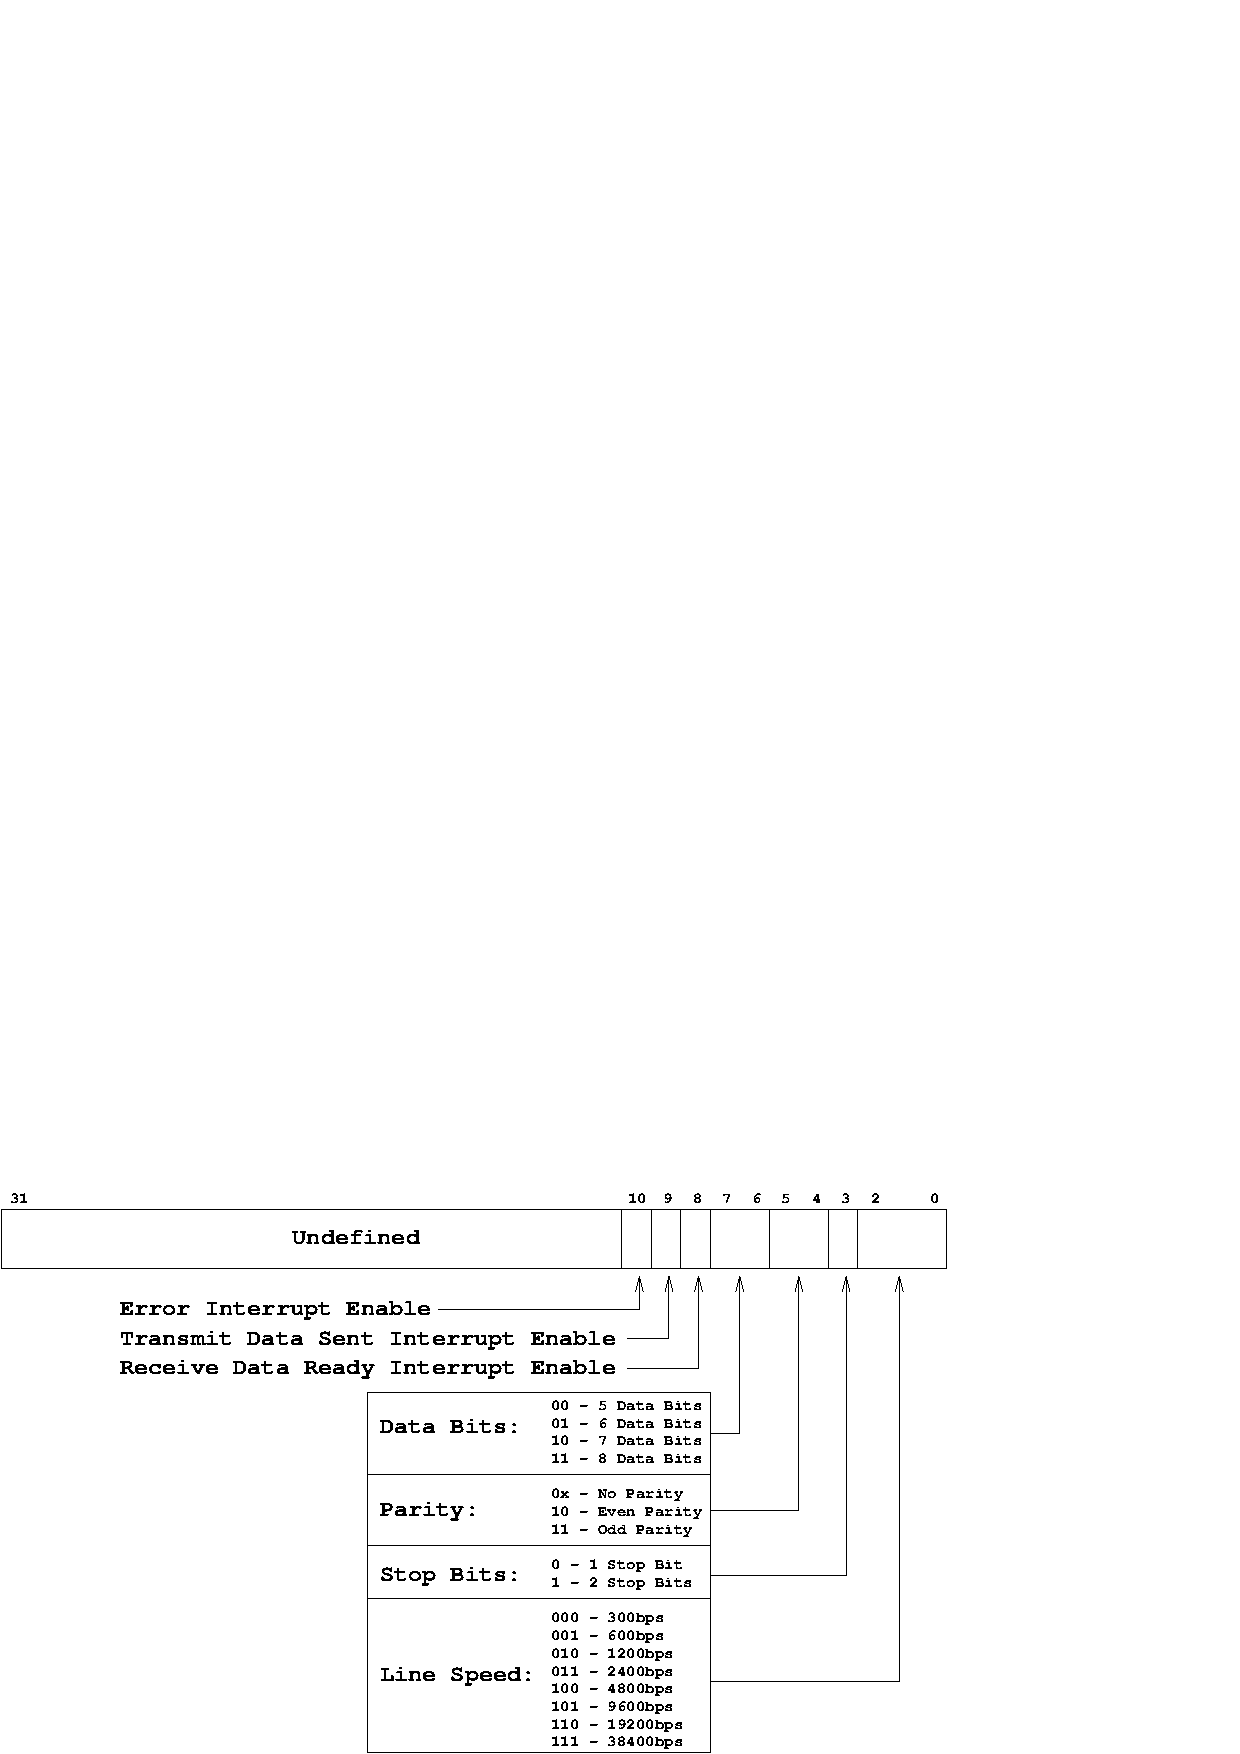
\includegraphics[width=0.8\textwidth]{serial_cr.pdf}
\caption{The Serial Control Register}
\label{serial_cr_pic}
\end{center}
\end{figure}

\noindent
eg. To configure a serial interface to operate with no interrupts
enabled, at 9600 bits per second, with 8 data bits, no parity and 1
stop bit, the value `\src{00011000101}' would be written to the
control register.

\subsection{Serial Status Register}

The status register is a read-only register, which gives error and
status information about the serial interface. It allows the
programmer to see if data has been received, sent, or if an error
condition is present.

The Transmit Data Sent (TDS) bit will be set to `\src{1}' as soon
as the transmit data register is empty. Checking that this bit is set
allows WRAMP code to ensure that it will not overwrite any data by
placing another character into the transmit data register. This bit
will automatically be cleared if the transmit data register becomes
full.

Similarly, the Receive Data Ready bit will be set to `\src{1}' as soon
as there is new valid data in the receive data register. A read from
the receive data register automatically clears this bit.

Note that while reading from the receive data register and writing to the
transmit data register will clear the corresponding bits in the status
register, they will not acknowledge any interrupts generated. The
relevant bits in the interrupt acknowledge register must still be
set to zero.

\begin{figure}[h]
\begin{center}
\includegraphics[width=0.8\textwidth]{serial_sr.pdf}
\caption{The Serial Status Register}
\label{serial_sr_pic}
\end{center}
\end{figure}

\noindent
eg. If the value `\src{00001}' was read from the status register
then we could determine that a character has been received without
error, and is available in the receive data register.

\subsection{Serial Interrupt Acknowledge Register}

The interrupt acknowledge register is a read/write register. When the
serial interface has generated an interrupt this register allows the
program to determine the reason for the interrupt as well as
acknowledge interrupts that have been dealt with.

To acknowledge an interrupt a zero (`\src{0}') should be written
over the current status field for the type of interrupt being
acknowledged. Most often it will be the desire of the programmer to
acknowledge all of the possible serial port interrupts in one
instruction. This can be achieved by storing register \reg{0} to
the interrupt acknowledge register.

\begin{figure}[h]
\begin{center}
\includegraphics[width=0.8\textwidth]{serial_iack.pdf}
\caption{The Serial Interrupt Acknowledge Register}
\label{serial_iack_pic}
\end{center}
\end{figure}

\noindent
eg. If the value `\src{010}' was read from the interrupt
acknowledge register we could determine that the cause of the
interrupt was the transmit data register becoming empty. If the value
`\src{000}' was written to the interrupt acknowledge register all
outstanding serial port interrupts would be acknowledged.

\section{Parallel Interface}

The parallel interface on the Basys board provides an input interface
from a bank of 16 on-off switches and three momentary push-buttons, as
well as an output interface to four LED Seven Segment Displays (SSDs)
and 16 LEDs.
Parallel interrupts, if enabled, will be generated on any switch or
push-button state change.

The programmer's view of the parallel interface consists of 10
registers. The names of these registers and their addresses,
expressed as offsets from the base address, are provided in
Table~\ref{table:parallel_offsets}. The base address for the parallel
port is \src{\LOCPARABASE}. Please note that due to the inclusion of
two more SSDs in the Basys implementation, the original two SSDs can
be addressed from two locations to allow for both backwards compatibility
and to have all 4 SSDs in sequential addresses.

\begin{table}[h]
\begin{center}
\begin{tabular}{|l|c|}
\hline
\textbf{Register name} & \textbf{Offset} \\
\hline
Parallel Switch Register & 0 \\
\hline
Parallel Push Button Register & 1 \\
\hline
Parallel Lower Left SSD Register & 2 \\
\hline
Parallel Lower Right SSD Register & 3 \\
\hline
Parallel Control Register & 4 \\
\hline
Parallel Interrupt Acknowledge Register & 5 \\
\hline
Parallel Upper Left SSD Register & 6 \\
\hline
Parallel Upper Right SSD Register & 7 \\
\hline
Parallel Lower Left SSD Register & 8 \\
\hline
Parallel Lower Right SSD Register & 9 \\
\hline
Parallel LED Register & 10 \\
\hline
\end{tabular}
\caption{Parallel Port Register Offsets}
\label{table:parallel_offsets}
\end{center}
\end{table}

\subsection{Parallel Switch Register}

The switch register is a read-only register. A read from this register
returns a bit pattern with bits set corresponding to the switches that
are on.

\begin{figure}[h]
\begin{center}
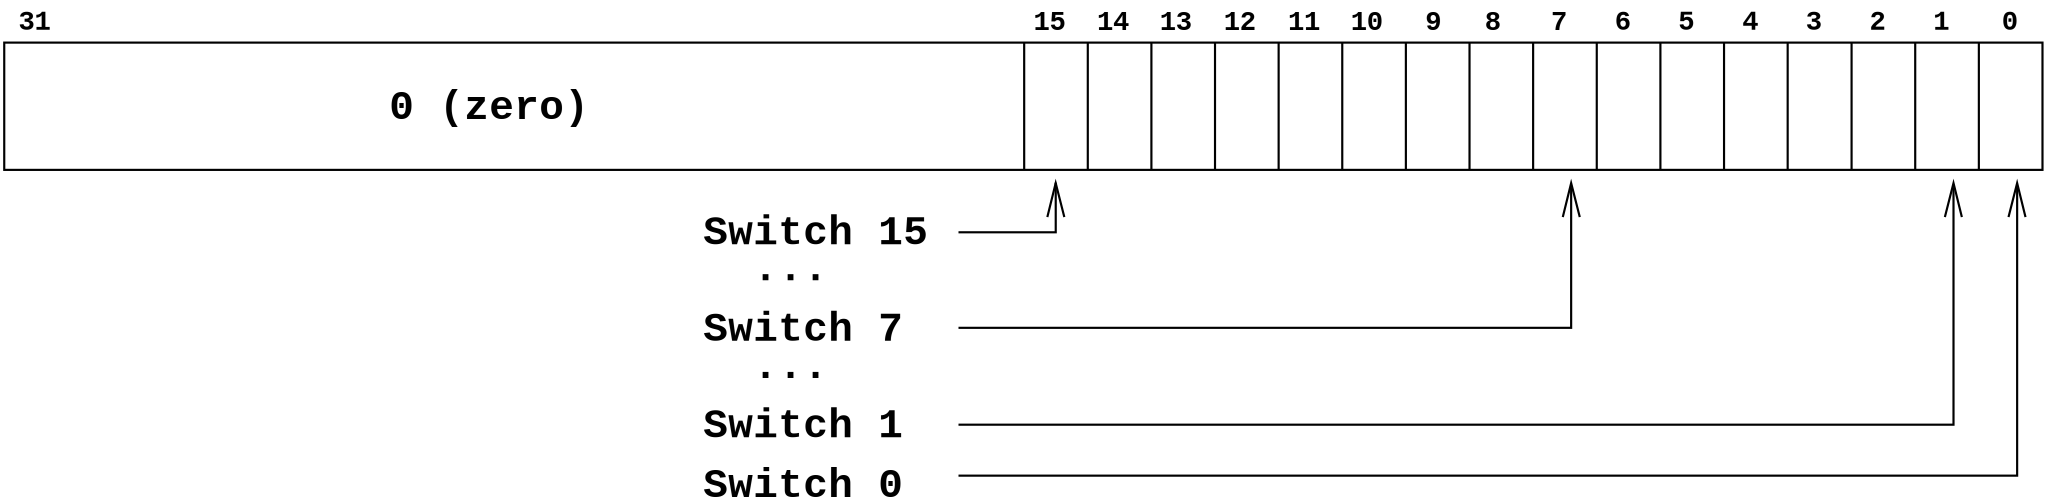
\includegraphics[width=0.8\textwidth]{switch_reg.pdf}
\caption{The Switch Register}
\label{switch_reg_pic}
\end{center}
\end{figure}


\subsection{Parallel Push Button Register}

The push button register is a read-only register. A read from this
register returns a bit pattern in the low order 3 bits corresponding
to the push buttons that are currently being depressed.

\begin{figure}[h]
\begin{center}
\includegraphics[width=0.8\textwidth]{button_reg.pdf}
\caption{The Push Button Register}
\label{button_reg_pic}
\end{center}
\end{figure}

\subsection{Parallel Left, Right, Upper and Lower SSD Registers}

The four SSD Registers are read/write registers. These
registers contain the value to be displayed on their respective Seven
Segment Display. 

If the hexadecimal to seven-segment decode bit is enabled in the
parallel control register, four bits of input will be decoded into a
single hexadecimal digit and displayed on the seven-segment display.

If the hexadecimal to seven-segment decode bit is turned off, then
each segment can be individually controlled by a single bit of the
input. The displays are made up of seven segments and a decimal point.
The first eight bits of input turn on the segments as shown in
Figure~\ref{fig:ssd}.
Hex-decode is enabled by default.

\begin{figure}[h]
\begin{center}
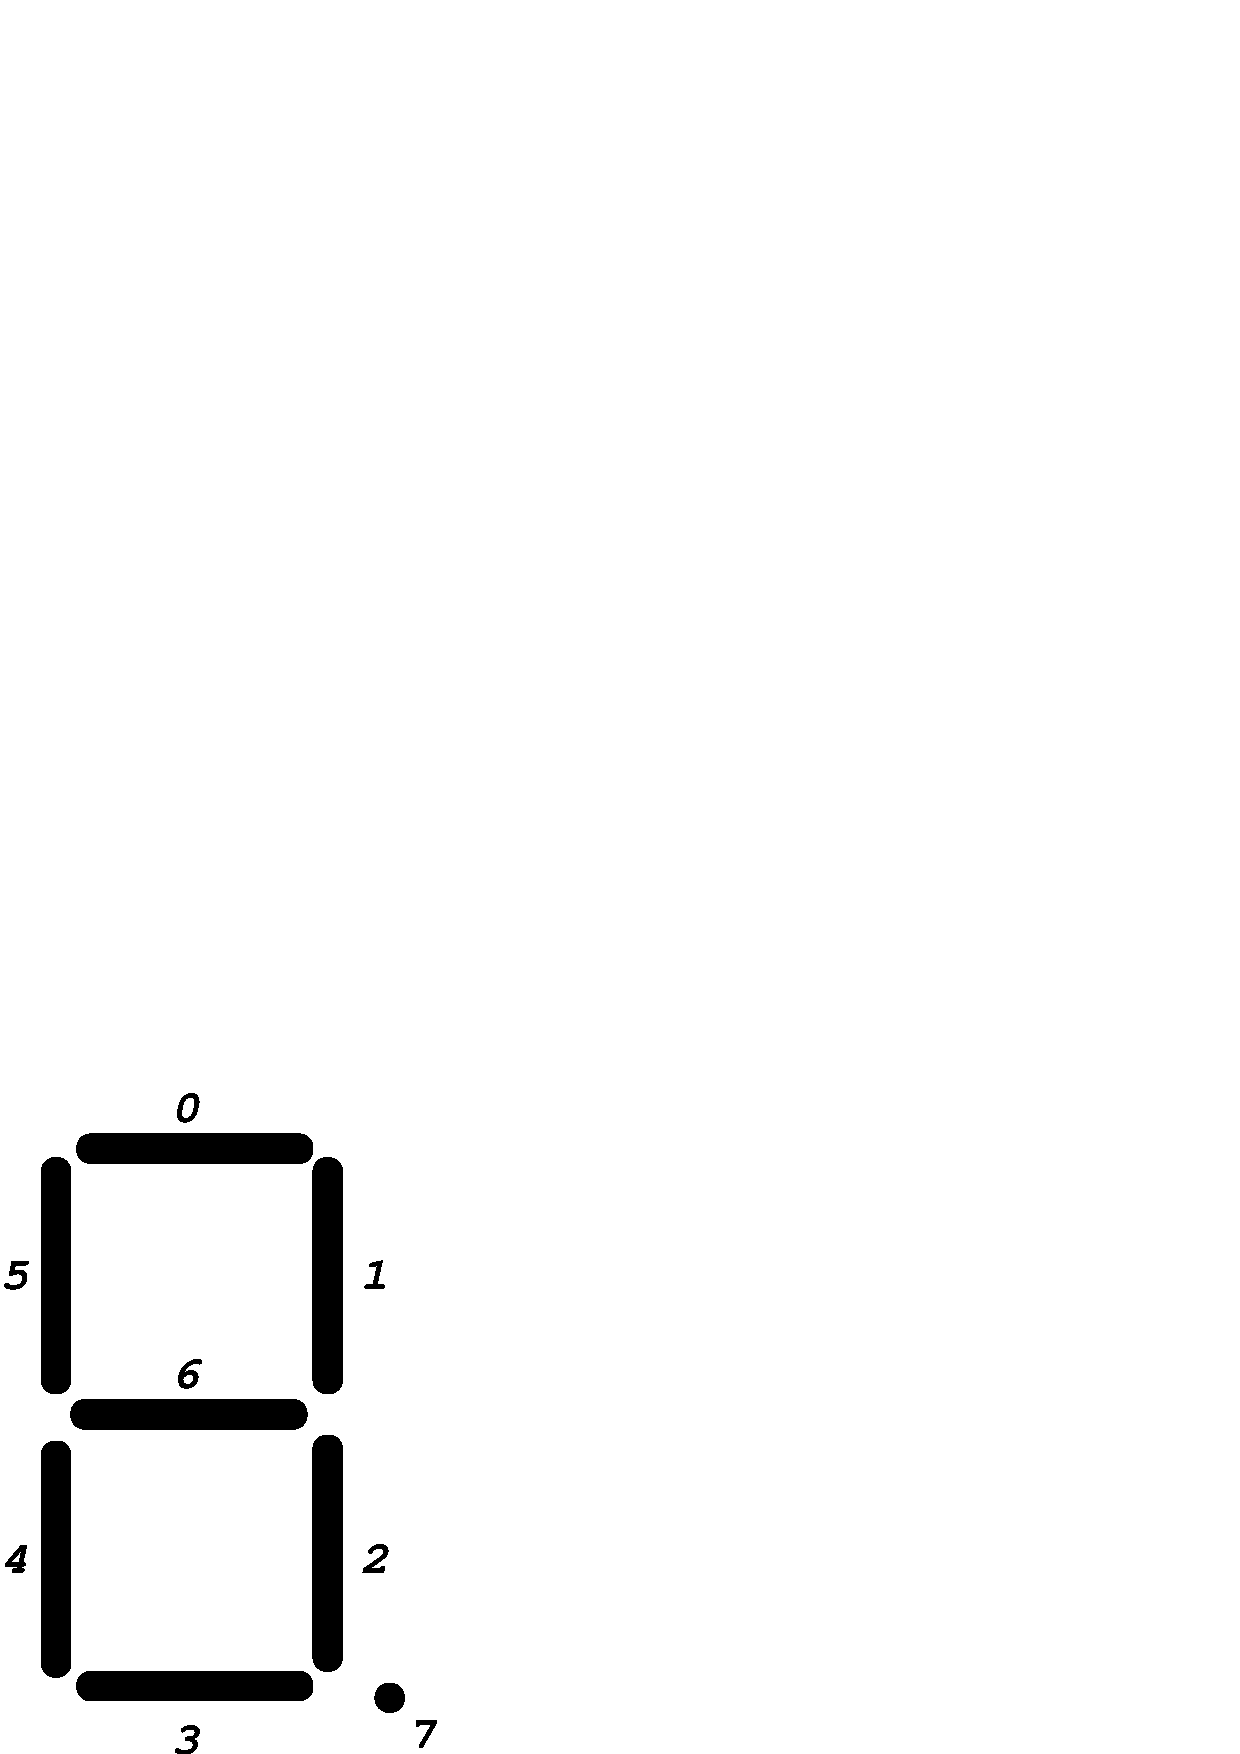
\includegraphics[width=0.12\textwidth]{ssd.pdf}
\caption{Seven-segment display bit encoding}
\label{fig:ssd}
\end{center}
\end{figure}

In this manual, the terms Upper and Lower refer to the left and right
pairs of SSDs respectively. As such, the far left SSD is the Upper Left
SSD (addressed with offset 6), and the second from the left is the Lower
Left SSD (addressed with either offset 8 or 2).

\begin{figure}[h]
\begin{center}
\includegraphics[width=0.3\textwidth]{ssd_layout.pdf}
\caption{SSD Layout}
\label{ssd_layout_pic}
\end{center}
\end{figure}

\subsection{Parallel Control Register}

The Parallel Control Register is a read/write register, which allows
for control over the parallel interface.

\begin{figure}[h]
\begin{center}
\includegraphics[width=0.8\textwidth]{parallel_cr.pdf}
\caption{The Parallel Control Register}
\label{parallel_cr_pic}
\end{center}
\end{figure}

eg. To enable interrupts on switch changes and force hex-SSD decoding
on the displays, a value of `\src{11}' would be written to
the parallel control register.

\subsection{Parallel Interrupt Acknowledge Register}

The Interrupt Acknowledge Register is a read/write register. This
register allows a program to determine the parallel port interrupt
status as well as acknowledge interrupts that have been dealt with.

\begin{figure}[h]
\begin{center}
\includegraphics[width=0.8\textwidth]{parallel_iack.pdf}
\caption{The Parallel Interrupt Acknowledge Register}
\label{parallel_iack_pic}
\end{center}
\end{figure}

eg. To acknowledge an outstanding parallel port interrupt `\src{0}'
would be written to the parallel interrupt acknowledge register.

\subsection{LED Register}

The LED register is a read/write register. This
register allows a program to selectively illuminate the bank of 16 LEDs
sitting above the switches.

\begin{figure}[h]
\begin{center}
\includegraphics[width=0.8\textwidth]{led_reg.pdf}
\caption{The LED Register}
\label{LED_pic}
\end{center}
\end{figure}

\section{Programmable Timer}

The Programmable Timer on the Basys board allows for the generation of
interrupts at time intervals from about 1ms to 30s, with a resolution
of around 0.5ms.

The timer has an internal 16-bit register. This register is decremented
at a constant rate of 2400Hz. Once this register reaches
\src{0x0000} an interrupt is triggered. The starting value for the
timer is controlled by altering the value in the timer load register.

Please note due to the new hardware, a rate of exactly 2400Hz was not attainable.
Instead of picking another whole number, the clock rate was approximated
to maintain backwards compatibility. Internally, a register counts down from 1302 
at a rate of 6.25MHz, then inverts a clock signal to the timer.
Every second inversion of this signal will decrement the timer's counter.
This yields an approximate ((6.25Mhz/1302)/2) = 2400.153609831Hz.
This has an error of approximately 5 seconds per 24 hours of timer operation.

The timer can be configured to automatically reload the starting count
value and continue counting immediately after it expires.

The programmer's view of the timer consists of four registers.  The
names of these registers and their addresses, expressed as offsets
from the base address, are provided in
Table~\ref{table:timer_offsets}.  The base address for the timer is
\src{\LOCTIMEBASE}.

\begin{table}[h]
\begin{center}
\begin{tabular}{|l|c|}
\hline
\textbf{Register name} & \textbf{Offset} \\
\hline
Timer Control Register & 0 \\
\hline
Timer Load Register & 1 \\
\hline
Timer Count Register & 2 \\
\hline
Timer Interrupt Acknowledge Register & 3 \\
\hline
\end{tabular}
\caption{Timer Register Offsets}
\label{table:timer_offsets}
\end{center}
\end{table}

\subsection{Timer Control Register}

The Timer Control Register is a read/write register, that allows the
user to enable and control aspects of the timer operation. The timer
has two primary modes of operation, automatic restart and single-shot
mode. If the timer is set to automatic restart, as soon as the timer
expires, an interrupt is triggered and the timer immediately starts
counting down again. In single-shot mode the timer will copy the value
from the timer load register only once when the timer is enabled and
will count down to zero. Once the timer reaches zero an interrupt will
be triggered and the timer will be disabled.

\begin{figure}[h]
\begin{center}
\includegraphics[width=0.8\textwidth]{timer_cr.pdf}
\caption{The Timer Control Register}
\label{timer_cr_pic}
\end{center}
\end{figure}

\subsection{Timer Load Register}

The Timer Load Register is a read/write register. This register allows
the user to specify the starting count value. The starting count value
is a 16-bit value with the upper 16 bits being ignored.

\subsection{Timer Count Register}

The Timer Count Register is a read-only register. Reading from this
register returns the current value in the 16-bit internal count
register.

\subsection{Timer Interrupt Acknowledge Register}

The Interrupt Acknowledge Register is a read/write register. This
register allows a program to detect a timer overrun as well as
acknowledge interrupts that have been dealt with.

The overrun detected bit will be set if the timer is set to automatic
restart and the timer expired again before the previous interrupt was
acknowledged. This allows a program to detect if it is unable to
service the timer interrupt fast enough.

The overrun bit must be manually reset by writing a `\src{0}' to
it's location.

\begin{figure}[h]
\begin{center}
\includegraphics[width=0.8\textwidth]{timer_iack.pdf}
\caption{The Timer Interrupt Acknowledge Register}
\label{timer_iack_pic}
\end{center}
\end{figure}

eg. If the value `\src{11}' was read from the interrupt acknowledge
register we could determine that the timer has overrun since we last
acknowledged an interrupt. If `\src{00}' was written to the timer
interrupt acknowledge register we will acknowledge any outstanding
interrupts and ensure the overrun bit is reset to zero.

\subsection{Timer Example}

To configure the timer to interrupt at a specific period the first
step is to calculate the timer load value. This value can be
calculated simply by multiplying the timer frequency by the required
time between interrupts. For example, if we want the timer to generate
an interrupt once every ten seconds we would calculate it as follows:

\begin{center}
Timer Load = 2400Hz * 10s = 24000 = 0x5dc0
\end{center}

Some simple code to initialise the timer to automatically restart and
interrupt once every ten seconds is given in
Figure~\ref{code:timer_init}.

\begin{figure}[h]
\begin{footnotesize}
\begin{center}
\begin{tabular}{|p{8cm}|}
\hline
\begin{verbatim}
            . . .
           # Make sure there are no old interrupts
           # still hanging around
           sw   $0, 0x72003($0)
           # Put our auto load value in
           addi $11, $0, 0x5dc0
           sw   $11, 0x72001($0)
           # Enable the timer and autorestart
           addi $11, $0, 0x3
           sw   $11, 0x72000($0)
            . . .
\end{verbatim}
\\
\hline
\end{tabular}
\end{center}
\end{footnotesize}
\caption{Simple Timer Initialisation}
\label{code:timer_init}
\end{figure}

\chapter{Exceptions}
\label{chapter:exceptions}
\section{Introduction}

Modern processors can execute millions of instructions each
second. This means that when a processor is polling an I/O device for
data or status information which may only change very infrequently, it
is wasting a lot of time where it could be doing some worthwhile
processing.  It would be more efficient for a device to signal the CPU
when something happens (eg. a character is received at the serial
port, the user flicks a switch, or a certain time has elapsed).

Also consider what should happen if something goes wrong when a
program is executing. What should happen if an attempt is made to
divide by zero? What should happen if you add two numbers and the
result will not fit in 32 bits?

This is why almost all modern processors provide support for
exceptions. Exceptions provide a mechanism which allows the processor
to be executing code, and when a certain condition occurs, to deal
with that condition, and then return to what it was doing initially.

The terms `exception' and `interrupt' are often used
interchangeably. There are varying opinions on the exact definitions of
these terms, however the term `interrupt' generally refers only to the
exceptions which are caused by something outside the processor
(eg. the serial port, or the timer).

The WRAMP processor allows for four internal exceptions. These are:

\begin{itemize}
\item Arithmetic Exception (ie. Divide-by-zero, or Overflow)
\item Breakpoint Exception (a 'break' instruction has been executed)
\item System Call Exception (a 'syscall' instruction has been
executed)
\item General Protection Fault Exception (eg. an illegal instruction
is encountered)
\end{itemize}

WRAMP provides eight external interrupts. The external interrupts are 
simply wires coming into the processor, and so can be connected to any 
devices.  These are called IRQ0 (for Interrupt ReQuest) to IRQ7. On the 
Basys board these are connected as follows:

\begin{center}
\begin{tabular}{|c|l|c|l|}
\hline
\textbf{IRQ \#} & \textbf{Description} & \textbf{IRQ \#} &
\textbf{Description} \\
\hline
0 & Unconnected & 4 & Serial Port 1 Interrupt \\
\hline
1 & User Interrupt Button & 5 & Serial Port 2 Interrupt\\
\hline
2 & Timer Interrupt & 6 & Unconnected \\
\hline
3 & Parallel Interrupt &7 & Unconnected \\
\hline
\end{tabular}
\end{center}

Exceptions can be thought of as similar to subroutine calls. The
processor is executing a block of code, when an exception occurs,
causing the processor to jump to a location called the `exception
vector'.  The processor then executes the code at this location (known
as the `exception handler' or `exception routine'), and returns to the
point at which it was executing when the exception occurred.

For this mechanism to work, we will need registers to store things
like the exception vector (the address of the exception handler), and
the address of the instruction to return to after the exception has
been handled. The general purpose registers are not suitable for this,
because a program may be using them, and if an exception occurs, then
there may be unpredictable results. For this reason the WRAMP
processor provides a special set of registers that are used for
advanced processor features like exceptions.

Like the general purpose registers (\reg{0} - \reg{ra}), there are 16 special
purpose registers. Because each has a specific use, they are called by
their names rather than their numbers. The special registers concerned
with exceptions are:

\begin{itemize}
\item \reg{cctrl} - CPU Control Register
\item \reg{estat} - Exception Status Register
\item \reg{evec} - Exception Vector Register
\item \reg{ear} - Exception Address Register
\item \reg{ers} - Exception Register Save
\end{itemize}

All special purpose registers cannot be operated on directly like
the general purpose registers. Rather, two instructions are provided
to allow register contents to be copied from a general purpose
register to a special purpose register, or vice-versa. These
instructions are \src{movsg} (move special register to general
register), and \src{movgs} (move general register to special
register). Details on these instructions can be found in the WRAMP
instruction reference in Appendix \ref{appendix:instr}.

The next sections will describe the format of each of these special
purpose registers. Contained in these descriptions will often be
introductions to new concepts and ideas. As such this chapter is best
read once end-to-end to ensure that all concepts are introduced fully.

\section{CPU Exception Control Registers}

\subsection{\$cctrl - CPU Control Register}

\begin{figure}[h]
\begin{center}
\includegraphics[width=\textwidth]{cctrl.eps}
\caption{\$cctrl - CPU Control Register}
\label{cctrl_pic}
\end{center}
\end{figure}

The CPU control register controls almost all of the functionality
related to the WRAMP exception mechanism. There are three main
sections of this register:

\begin{itemize}
\item Interrupt Enable (IE)
\item Kernel/User Mode (KU)
\item Interrupt Mask
\end{itemize}

\subsubsection{Interrupt Enable}

This flag provides a global interrupt enable. If this location is set
to `\src{0}' then no interrupts can be triggered. This flag
\emph{only} affects external interrupts. There is no way on the WRAMP
processor to disable internal exceptions.

Interrupts that occur while the global interrupt enable is turned off
will be held back. As soon as interrupts are again enabled by writing
a `\src{1}' into this location the interrupt mask will be consulted
to discover if that specific interrupt is enabled. See
Section~\ref{sec:imask} for more information about the interrupt mask.

The CPU will automatically set the IE bit to `\src{0}' whenever an
exception of any type occurs. This prevents the exception handler
from being interrupted by another interrupt.

\subsubsection{Interrupt Mask}
\label{sec:imask}

This provides a way to selectively turn on and off individual external
interrupts. This field has a bit corresponding to each of the eight
possible external interrupts (IRQ0 - IRQ7). Bit 4 of the CPU control
register corresponds to IRQ0, bit 5 to IRQ1 and so on.

The interrupt mask field is only consulted if the global interrupt
enable (IE) flag is set. If an interrupt occurs and the global
interrupt flag is set but the individual interrupt mask is disabled
then the interrupt will be held back. As soon as both the global
interrupt enable and the specific interrupt mask bits are set then the
interrupt will occur.

\subsubsection{Kernel User Mode}

The WRAMP CPU has two modes of operation, kernel and user mode. If
there is a `\src{1}' in the KU bit the CPU is in kernel mode. If
the KU bit is set to `\src{0}' then the CPU is in user mode. 

If the CPU is running in kernel mode it will execute all instructions and
allow access to all areas of memory. If the CPU is running in user
mode programs are not allowed to use any of the three instructions
which deal with the special register file (\src{movsg, movgs, rfe})
and may not be able to access all memory locations. If a program
running in user mode attempts to use one of these instructions, or to
access protected memory the CPU will cause a General Protection Fault
exception. %TODO see section on the MPU

The CPU will automatically set the KU bit to `\src{1}' whenever an
exception of any type occurs. This allows the exception handler to
operate in kernel mode, allowing it full access to all instructions
and memory locations.

\subsection{\$estat - Exception Status Register}

\begin{figure}[h]
\begin{center}
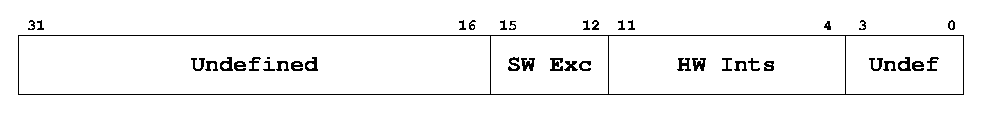
\includegraphics[width=\textwidth]{estat.eps}
\caption{\$estat - Exception Status Register}
\label{estat_pic}
\end{center}
\end{figure}

The exception status register provides the exception handler with the
ability to discover which exceptions caused it to be invoked. The
exception status register has a single bit flag for each external IRQ
line. Bit 4 of the status register corresponds to IRQ0, bit 5 to IRQ 1
and so on. These locations are exactly the same as the locations of
the interrupt mask fields in the CPU control register as described in
Section~\ref{sec:imask}. In addition to the eight external interrupt
sources the status register also provides the status for the four CPU
internal exception sources. 

The full list of all exception sources and their related status
register bit is given in Table~\ref{table:sta_loc}.

Most exception handlers will wish to check which exception caused them
to be called. Provided in Figure~\ref{code:stat_check} is code that
checks if a specific interrupt caused the handler to be called. If any
other interrupt or exception is currently high then the code will call
an old handler to deal with the exception. The code to save the
address of an old handler is given in Figure~\ref{code:evec} and
discussed in Section~\ref{sec:evec}.

\begin{table}[h]
\begin{center}
\begin{tabular}{|l|c|}
\hline
\textbf{Exception source} & \textbf{Bit location} \\
\hline
IRQ0 & 4 \\
\hline
IRQ1 - User Interrupt Button & 5 \\
\hline
IRQ2 - Timer Interrupt & 6 \\
\hline
IRQ3 - Parallel Interrupt & 7 \\
\hline
IRQ4 - Serial Port 1 Interrupt & 8 \\
\hline
IRQ5 - Serial Port 2 Interrupt & 9 \\
\hline
IRQ6 & 10 \\
\hline
IRQ7 & 11 \\
\hline
General Protection Fault Exception & 12 \\
\hline
System Call Exception & 13 \\
\hline
Breakpoint Exception & 14 \\
\hline
Arithmetic Exception & 15 \\
\hline
\end{tabular}
\caption{Exception Status Register Fields}
\label{table:sta_loc}
\end{center}
\end{table}

\begin{figure}[h]
\begin{footnotesize}
\begin{center}
\begin{tabular}{|p{10cm}|}
\hline
\begin{verbatim}
          . . .
  handler:

        # Get the status register
        movsg   $13, $estat

        # Inspect only the bits we are interested in. We want 
        # to check that no bits from the sw exceptions or 
        # hardware exceptions, other than the one we were 
        # expecting, are enabled.
        #
        # This code is looking for an IRQ4 interrupt.
        andi    $13, $13, 0xfef0
         
        # If the result of this is zero then no other 
        # exceptions are enabled so it must be our interrupt
        # that caused us to be called.
        beqz    $13, handle_interrupt 

        # Otherwise there was another exception that has 
        # occurred, so call the old handler
        lw      $13, old_vector($0)
        jr      $13

  handle_interrupt:

        # This is where we deal with the interrupt.
           . . .
\end{verbatim}
\\
\hline
\end{tabular}
\end{center}
\end{footnotesize}
\caption{Checking the Status Register}
\label{code:stat_check}
\end{figure}

\subsection{\$evec - Exception Vector Register}
\label{sec:evec}

When an exception occurs the CPU needs to jump to the exception
handler. The CPU must therefore know what address the exception
handler starts at.

The address of the exception handler is stored in the exception vector
register. The CPU jumps to this location whenever an exception occurs.

If a program is replacing an existing exception handler, but will still
need to call the old handler for certain exceptions, the code must
be careful to save the address of the old exception handler. This
allows the new handler to decide if it will deal with this exception,
and if not, call the old handler.

A section of WRAMP code to save the address of an old exception
handler, load the address of the new handler and save this to the
exception vector is given in Figure~\ref{code:evec}.

\begin{figure}[h]
\begin{footnotesize}
\begin{center}
\begin{tabular}{|p{8cm}|}
\hline
\begin{verbatim}
          . . . 
        # Get the old exception vector
        movsg   $4, $evec
        # And save it
        sw      $4, old_vector($0)

        # Get the address of our handler
        la      $4, handler
        # And put it in the exception vector register
        movgs   $evec, $4

            . . .
	
   handler:
        # The exception handler goes here

            . . .

   old_vector:
        .word   0

\end{verbatim}
%$
\\
\hline
\end{tabular}
\end{center}
\end{footnotesize}
\caption{Saving and Initialising the Exception Vector}
\label{code:evec}
\end{figure}

\subsection{\$ear - Exception Address Register}

An exception routine must be able to return to the point in program code at
which the exception occurred.  To allow this, when an exception occurs the
WRAMP pocessor automatically saves the address of the next instruction
that would have been executed into \reg{ear} - the Exception Address
Register.

When the exception routine has completed its processing, it executes a
Return From Exception, or \src{rfe} instruction. Amongst other things, this
instruction causes a jump to the address contained in \reg{ear}.

In some circumstances an exception routine may wish to know the address at
which the exception was invoked, or may wish to alter the address to which
the \src{rfe} will return. This can be achieved by inspecting and/or modifying
the contents of the \reg{ear}.

\subsection{\$ers - Exception Save Register}

It is vital that an exception routine does not change the contents of the
general purpose registers when it returns to the main program, as changes
may cause the main program to behave in an unpredictable fashion.

However, for the exception handler to determine the cause of the exception,
it requires a general purpose register into which it can copy
\reg{estat}. The WRAMP processor makes general purpose register \reg{13}
available for this by automatically copying it to the Exception Save
Register (\reg{ers}) when an exception occurs. The opposite of this happens
when an \src{rfe} instruction is executed - \reg{ers} is copied into
\reg{13}.

This means that exception handler code must only change \reg{13}.  If
it needs other registers it must save their contents before using
them.  They must then be restored before returning to the main
program.

\section{User Interrupt Button}

The Basys board provides a simple method for creating an
interrupt. There is a set of five buttons located on the bottom right.
The interrupt button is the bottom one. When this button is pressed IRQ1,
the ``User Interrupt Button'', interrupt will be triggered. If this
interrupt is unmasked and the global interrupt enable is turned on in
\src{\$cctrl} an exception will occur.

This button provides a simple way to test an exception handler as it
avoids problems that could be caused by mis-configuration of the I/O
device that is being used to provide the exception.

Like all other WRAMP interrupt sources the user interrupt button needs
to be acknowledged each time an exception occurs. To acknowledge a
``User Interrupt'' you store zero to the address
\src{0x7f000}. Unlike the other I/O devices on the Basys board you do
not need to enable or disable the user interrupt button. If IRQ1 is
unmasked in \src{\$cctrl} and interrupts are enabled the button
will cause an exception when pressed.

\section{Using Exceptions}

Writing a program that uses exceptions is best done as a step by step
process. If you attempt to write an entire program that uses exceptions
from start to finish in one hit, then there is a good chance you will never
debug any problems that may arise.

The first thing that you will need when writing your first handler is a
simple program that will run as the main loop of your code. You use this to
ensure that the exception routine is returning to your original code
correctly. A program which reads the value on the switches and writes this
to the seven segment display is ideal. Obviously you should do this in a
polled fashion.

Next you should write a very simple piece of code that will constitute
your exception handler. A suggested program is one which writes a
single character to a serial port. As this code will eventually be run
from inside your exception handler it must transmit this character
using polled I/O.

Test that both of these pieces of code work in a normal environment with no
exceptions. Also ensure that the code which will act as your exception
handler makes use only of \reg{13}.

The next step is to actually enable an interrupt and get the handler
you just wrote to be run. As suggested above the best source for your
first interrupt is the user interrupt button, IRQ1. The things that
you need to do to get this working are:

\begin{itemize}
\item Save the old exception handler address
\item Put the address of your new handler into \src{\$evec}
\item Make sure that there are no old interrupts hanging around by
storing \src{\$0} to the acknowledge register of the device you
will be using. For IRQ1 the acknowledge register is at address
\src{0x7f000}.
\item Configure the CPU control register to enable interrupts. This
takes a number of smaller steps:
\begin{itemize}
\item Get the current value of \src{\$cctrl}
\item Disable all interrupts.
\item Enable the interrupt you wish to use (IRQ1) and set the global
interrupt enable to `\src{1}'. Be careful that you do not alter any
other locations in this register besides the ones specified.
\item Store this value back into \src{\$cctrl}.
\end{itemize}
\end{itemize}


You will need to add some code to the simple exception handler that
you just wrote to make it a complete exception handler. Your exception
handler must start with code to detect if the interrupt is one that
you wish to deal with. Some example code for this is given in
Figure~\ref{code:stat_check}. Beware that you will need to alter this
code so that it checks for the correct interrupt. If you are using the
user interrupt button you should make sure the code checks that only
IRQ1 is high.

Next you must remember to acknowledge the interrupt. If you do not
acknowledge the interrupt then as soon as your exception routine exits
it will be instantly called again. This means you code will be stuck
in an infinite loop, probably printing character after character to
the serial port.

The very final instruction of you exception handler must be an
\src{rfe}. Only use an \src{rfe} instruction in code that you
are sure will only be called as part of an exception handler. If you
use the \src{rfe} instruction when you are not inside an exception
handler you may find your code will get stuck in an infinite loop or
crash.

If this code is now working, then you should have a character appearing
each time you push the user interrupt button as well as the value on the
switches constantly being displayed on the seven segment display. If so,
try altering your code so that you use one of the other I/O devices to
cause exceptions.

\section{Exception Procedure}

What actually happens when an exception occurs? The CPU performs a
number of operations when an exception occurs but they are all pretty
simple. The CPU does the following:

\begin{itemize}
\item Copy the IE bit into the OIE bit
\item Set IE to zero
\item Copy the KU bit into the OKU bit
\item Set KU to one
\item Set the \reg{estat} register to reflect the cause of the exception
\item Copy \reg{13} into \reg{ers}
\item Save the program counter into \reg{ear}
\item Set the program counter to the contents of \reg{evec}
\end{itemize}

At this point the next instruction is fetched. This instruction is the
first instruction of the exception handler and therefore the handler
is now running.

Once the exception handler has finished the final instruction it will
call will be an \src{rfe}. The CPU takes the following steps to
execute an \src{rfe} instruction:

\begin{itemize}
\item Set the IE bit to OIE
\item Set the KU bit to OKU
\item Copy \reg{ers} into \reg{13}
\item Set the program counter to the contents of \reg{ear}
\end{itemize}

This means that the next instruction fetched will normally be the
next instruction of the original code. The IE and KU bits will also
normally be restored to the value they had when the exception occurred.

\section{Compliant Exception Routine}

The exception proceedure above provides a mechanism whereby an exception routine
can run when an exception occurs and restore control to the main program without
affecting its operation.  In this way an exception routine can be general
purpose to be used during the operation of any program.  Such a routine should:

\begin{itemize}
\item Only use\reg{13} freely
\item Save the contents of any other register before using it.
\item Restore the saved contents of any other register before finishing
\item Ensure that the contents of the OIE bit, the OKU bit, \reg{ers} and
\reg{ear} are not modified
\item Finish with an \src{rfe}  instruction.
\end{itemize}

In addition any new exception routine that is installed must:

\begin{itemize}
\item Save the address of the system exception handler
\item Check the exception type
\item Pass any exceptions it cannot handle to the system exception handler
\end{itemize}

An exception routine that meets all these requirements is termed {\em compliant}
with the WRAMP conventions.

\section{Other Special Registers}

Although there are 16 special registers, the assembler requires they are called by name of which only 9 are named.
The five exception related registers mentioned at the start of this chapter and four more disscussed here.  
These four registers are not needed for normal use.
These are:

\begin{itemize}
\item \reg{icount} - CPU Instruction count Register
\item \reg{ccount} - CPU Clock Cycle count Register
\item \reg{ptable} - Protection Table Register
\item \reg{rbase} - User Base Register
\end{itemize}

Like the previous special registers, these cannot be operated on directly and can only be accessed with the \src{movsg} and \src{movgs} instructions.

\subsection{\reg{icount} - CPU Instruction count Register}
The \reg{icount} register keeps a running tally of the number of instructions executed since the last restart.

\subsection{\reg{ccount} - CPU Clock Cycle count Register}
The \reg{ccount} keeps count of how many clock cycles have elapsed since the last restart.
The clock rate is \src{6.25MHz}, or \src{0.00000016s} per cycle (\src{160ns}).
Please note that not all instructions take the same number of clock cycles to execute, and that kernel/user mode can also change the number of cycles per instruction.

\subsection{\reg{ptable} - Protection Table Register}
The \reg{ptable} register specifies the location of the protected memory table, which is 32 words in size.
Each word represents \src{32,768} (\src{0x8000}) memory locations, and each bit represents \src{1,024} (\src{0x400}) memory locations.
If the bit is zero then the associated memory location is protected and cannot be accessed in user mode.
A GPF will be thrown if this is attempted.
During the setup stage of WRAMPmon, the protection table will be initialized to the top of RAM and set so that all memory is accessible.

For example, if \reg{ptable} is set to \src{0x200} and the data at location \src{0x200} was equal to \src{0xA0000000} then any memory accesses in the range \src{0x0}-\src{0x3FF} and \src{0x800}-\src{0xBFF} would be valid, but others would cause a GPF if accessed in user mode.

\subsection{\reg{rbase} - User Base Register}
The \reg{rbase} register was intended to be used to create virtual memory functionality.
However this was never fully implemented, its value is simply added to the address of any memory access.
WRAMPmon and many instructions do not account for this.
Thus modifying the \reg{rbase} register will break any instruction involving memory (including fetching new instructions to execute) and it is highly advised that this register is not touched.

\appendix
\chapter{The WRAMP Toolchain}
\label{appendix:wasm-wlink}
\setcounter{secnumdepth}{0}

\section{\wasm\ and \wlink}

\wasm\ and \wlink\ are the \BI{assembler} and \BI{linker} for WRAMP code,
respectively. \wasm\ receives a file containing WRAMP assembly code and
outputs an object file, while \wlink\ receives a set of object files
and outputs a linked program, in the Motorola S-record file format which
\WRAMPmon\ can receive.

An additional program, named \trim, can be used to convert an S-record
into a \filename{.mem} file, which can be used in the Xilinx Vivado Design
Suite when developing \WRAMPmon\ itself. \trim\ does not need to be
used for general WRAMP development, but is documented here for completeness.

This section details the usage and capabilities of these programs, as well as
some information on the file formats themselves.

\subsection{Command Line Usage}

The basic usage of each tool is quite simple. With the programs accessible by
a command line, their help notes can be seen by simply running them with no
arguments, such as in the following examples.

\begin{verbatim}
     $ wasm
     USAGE: wasm [-o output] file
     $ wlink
     USAGE: wlink [-Ttext address] [-Tdata address] [-[T|E]bss address] [-v] 
            [-o output] file1 file2 ...
\end{verbatim}

It can be seen that \wasm\ takes a single filename for a file containing
WRAMP assembly as a command-line argument, and will optionally accept a
\src{-o output} parameter, which allows you to specify an output file. By 
default, the output file will be created in the same directory as the input
file and given the same name, but with the file extension replaced with
\filename{.o} if the name ends with \filename{.s} or \filename{.S}. If it
ends with something else, \filename{.o} will be appended. As such, the
convention is for WRAMP assembly files to be given the \filename{.s} or
\filename{.S} extension.

\wlink\ can accept more complicated arguments, but the basic usage is
the same as for \wasm. The optional \src{-o output} parameter will set
the output file in the same fashion as \wasm. If omitted, the output file
will default to being named \filename{link.out} in the current working
directory. The rest of the arguments are considered input files, which should
all be object files as created by \wasm.

If \wlink\ is given a \src{-Ttext}, \src{-Tdata}, or \src{-[T|E]bss} argument, 
it will place the \BI{top} of the given segment at the address specified. For
example, if \src{-Ttext 0x10} is given, the first instruction in the
\src{.text} segment will be at address 0x10. The same applies for the
\src{.data} segment, and the \src{.bss} segment if \src{-Tbss} is given. If
\src{-Ebss} is given instead, the \src{.bss} segment will \BI{end} at the
address specified.

Finally, \wlink\ supports a \src{-v}, or \BI{verbose} option. Including this
option makes \wlink\ output additional information about the resulting
\filename{.srec} file. An example of a simple program that sets the values
of the LEDs and seven-segment displays to the state of the switches is shown
in Figure \ref{wlink-output}.

\wlink\ first prints a disassembly of the \src{.text} segment of the entire
program, after reordering the \src{.text} segments from each input file in the
order they were given on the command line. Each file has a separate header
specifying what address that segment begins at in the final program. The
disassembly is given, making it more easy to see which instruction ended up
where. This is useful when combined with \WRAMPmon's debugging commands,
detailed in Section \ref{intro:debugging}.

A display of the \src{.data} segments follows. This is a simple list of any
information placed in that section of each file, in the form it will appear
in memory. The example above shows the string \src{Hello!}. Finally, the
size of each file's \src{.bss} segment is displayed, followed by a summary
of each segment.

\begin{figure}[btp]
\begin{center}
\begin{tabular}{|p{15cm}|}
\hline
\begin{verbatim}
     $ wlink -v -o four-sevensegs.srec four-sevensegs.o
     file `four-sevensegs.o', starting : 0x00000, .text
     0x00000 : 81073000    lw	$1,0x73000($0)
     0x00001 : 9107300a    sw	$1,0x7300a($0)
     0x00002 : 121bf000    andi	$2,$1,0xf000
     0x00003 : 122c000c    srli	$2,$2,0x000c
     0x00004 : 131b0f00    andi	$3,$1,0x0f00
     0x00005 : 133c0008    srli	$3,$3,0x0008
     0x00006 : 141b00f0    andi	$4,$1,0x00f0
     0x00007 : 144c0004    srli	$4,$4,0x0004
     0x00008 : 151b000f    andi	$5,$1,0x000f
     0x00009 : 1a000001    addi	$10,$0,0x0001
     0x0000a : 9a073004    sw	$10,0x73004($0)
     0x0000b : 92073006    sw	$2,0x73006($0)
     0x0000c : 93073007    sw	$3,0x73007($0)
     0x0000d : 94073008    sw	$4,0x73008($0)
     0x0000e : 95073009    sw	$5,0x73009($0)
     0x0000f : 40000000    j	0x00000
     
     file `four-sevensegs.o', starting : 0x00010, .data
     0x00010 : 00000048    
     0x00011 : 00000065    
     0x00012 : 0000006c    
     0x00013 : 0000006c    
     0x00014 : 0000006f    
     0x00015 : 00000021    
     0x00016 : 00000000    

     file `four-sevensegs.o', starting : 0x00010, .bss : 0 words.

     entry point : 0x00000
     .text segment size = 0x00000010
     .data segment size = 0x00000007
     .bss segment size = 0x00000000
\end{verbatim}
\\
\hline
\end{tabular}
\end{center}
\caption{Example \wlink\ output for a simple program}
\label{wlink-output}
\end{figure}

\trim\ takes the same arguments as \wasm, but the input should be an
\src{.srec} file such as one generated by \wlink, and the output will default
to the \src{.mem} file extension.

\section{WRAMP File Formats}

There are three file formats which are used for all development of WRAMP
programs: \filename{.s}, \filename{.o}, and \filename{.srec}.
A \filename{.s} file contains WRAMP assembly source code, and is assembled into
a \filename{.o} \BI{object file}. One or several object files can be linked by
\wlink\ into an \filename{.srec} file, ready to be loaded into \WRAMPmon.

For projects containing mixed C and assembly code, it may be useful to follow
a slightly different convention. One such convention (used in the \WRAMPmon\ 
source code) is that assembly and object files which are not generated by a
tool, but are instead written or hand-picked by the user have a capitalised
file extension (\filename{.S} or \filename{.O}). This makes it clear which
files can be safely deleted, such as in a Makefile's \src{make clean} target.

\subsection{\wobj\ and \wdis}

Two tools exist which are able to inspect object and S-Record files: \wobj\
and \wdis. They should each be provided a single file of the correct format as
a command line argument.

\wobj\ will provide some details about object files, presented in a readable
format. The first section shows the \BI{symbol table}, which is a listing of
all global or undefined labels found in the source file. This could, for
example, be used to discover what functions a pre-assembled library offers.

The second section is the \BI{relocation table}, which shows where certain
parts of instructions will be replaced with other properties, such as the
address of a label. This will not show any unresolved labels.

Finally, a disassembly of the \src{.text} and \src{.data} segments is
displayed, in a similar fashion to the disassemblies offered by \wlink\ and
\WRAMPmon.

\wdis\ is able to disassemble an \filename{.srec} file. Its output is also
comparable to that of \wlink\ and \WRAMPmon.


\chapter{WRAMP Assembly Features}
\label{appendix:wramp-assembly}
\chapter{WRAMP Instruction Set Description}
\label{appendix:instr}
\setcounter{secnumdepth}{0}

\section{WRAMP General Purpose Registers}

\begin{small}
The WRAMP general purpose register file consists of 16 registers, each
being 32 bits wide. The hardware imposes special uses on only two of
these. Certain software register use conventions have been applied to
some of the remaining registers, but in essence, they remain true
general purpose registers, as the hardware does not restrict their
use.
\end{small}

\vspace{-4ex}
\begin{figure}[h]
\begin{center}
\begin{tabular}{|l|l|}
\multicolumn{1}{@{}p{4ex}}{}
& \multicolumn{1}{@{}p{50ex}}{}\\
\hline
Register &Description\\
\hline
\texttt{\$0} & Hardwired zero\\
\texttt{\$1} - \texttt{\$13} & General purpose registers\\
\texttt{\$sp} & Stack pointer\\
\texttt{\$ra} & Return address register\\
\hline
\end{tabular}
\end{center}
\caption{The WRAMP General Purpose Registers}
\label{wramp_regs}
\end{figure}

\begin{small}
Register zero (denoted \texttt{\$0}) always contains the value
zero. Any writes to this register have the value discarded. This
provides a constant source of zero that can be used for comparing and
initialising registers.

The fourteenth register is denoted \texttt{\$sp}. This register is
defined by the conventions to be the stack pointer. While the hardware
imposes no special conditions on this register, failure to follow this
convention may affect the ability of code to interoperate with other
software.

The fifteenth register is denoted \texttt{\$ra}. It is defined to be
the subroutine return address register. When a jump and link
instruction is executed this register is loaded with the address of
the next instruction after the jump and link. A return from subroutine
is performed by executing a jump to register \texttt{\$ra},
ie. \texttt{jr \$ra}.
\end{small}

\section{WRAMP Instruction Set Architecture}
\begin{small}
This section contains the details of the WRAMP instruction set. All
machine instructions are listed, with their encoding and a brief
description of their function. The instructions are grouped into
arithmetic instructions, bitwise instructions, test instructions,
branch instructions, memory instructions, and special instructions.

Each CPU instruction is a word (32 bits) in length. An instruction is
encoded in one of the three formats shown in figure
\ref{insn_encoding_formats}.
\end{small}

\newpage
% This is the table with the three instruction encoding formats
\begin{figure}[h]
{\bf I-Type instruction}
\itypeinsnformat
{\bf R-Type instruction}
\rtypeinsnformat
{\bf J-Type instruction}
\jtypeinsnformat
\vspace{1ex}
\begin{tabbing}
xxxx\=field name xxxxxxxx\=description \kill
\>\texttt{OPCode}\>4 bit operation code\\
\>\texttt{\regd{}}\>4 bit destination register specifier\\
\>\texttt{\regs{}}\>4 bit source register specifier\\
\>\texttt{\regt{}}\>4 bit source register specifier\\
\>\texttt{Func}\>4 bit function specifier\\
\>\texttt{Immediate}\>16 bit immediate field\\
\>\texttt{Address / Offset}\>20 bit absolute or relative address field
\end{tabbing}
\caption{WRAMP Instruction encoding formats}
\label{insn_encoding_formats}
\end{figure}


\subsection{Arithmetic Instructions}
\noindent
{\bf Addition}\\
\noindent
\texttt{add \regd, \regs, \regt}
\rtypeinsn{0000}{\regd}{\regs}{0000}{\regt}
Put the sum of register \regs{} and register \regt{}
into register \regd{}. Generate an overflow exception on signed overflow.
\vspace{3ex}

\noindent
{\bf Addition, immediate}\\
\noindent
\texttt{addi \regd, \regs, Immediate}
\itypeinsn{0001}{\regd}{\regs}{0000}{Immediate}
Put the sum of register \regs{} and the sign-extended immediate
into register \regd{}. Generate an overflow exception on signed overflow.
\vspace{3ex}

\noindent
{\bf Addition, unsigned}\\
\noindent
\texttt{addu \regd, \regs, \regt}
\rtypeinsn{0000}{\regd}{\regs}{0001}{\regt}
Put the sum of register \regs{} and register \regt{}
into register \regd{}. Generate an overflow exception on unsigned overflow.
\vspace{3ex}
\newpage

\noindent
{\bf Addition, unsigned, immediate}\\
\noindent
\texttt{addui \regd, \regs, Immediate}
\itypeinsn{0001}{\regd}{\regs}{0001}{Immediate}
Put the sum of register \regs{} and the zero-extended immediate
into register \regd{}. Generate an overflow exception on unsigned overflow.
\vspace{3ex}

\noindent
{\bf Subtraction}\\
\noindent
\texttt{sub \regd, \regs, \regt}
\rtypeinsn{0000}{\regd}{\regs}{0010}{\regt}
Put the difference of register \regs{} and register \regt{}
into register \regd{}. Generate an overflow exception on signed overflow.
\vspace{3ex}

\noindent
{\bf Subtraction, immediate}\\
\noindent
\texttt{subi \regd, \regs, Immediate}
\itypeinsn{0001}{\regd}{\regs}{0010}{Immediate}
Put the difference of register \regs{} and the sign-extended immediate
into register \regd{}. Generate an overflow exception on signed overflow.
\vspace{3ex}

\noindent
{\bf Subtraction, unsigned}\\
\noindent
\texttt{subu \regd, \regs, \regt}
\rtypeinsn{0000}{\regd}{\regs}{0011}{\regt}
Put the difference of register \regs{} and register \regt{}
into register \regd{}. Generate an overflow exception on unsigned overflow.
\vspace{3ex}

\noindent
{\bf Subtraction, unsigned, immediate}\\
\noindent
\texttt{subui \regd, \regs, Immediate}
\itypeinsn{0001}{\regd}{\regs}{0011}{Immediate}
Put the difference of register \regs{} and the zero-extended immediate
into register \regd{}. Generate an overflow exception on unsigned overflow.
\vspace{3ex}

\noindent
{\bf Multiplication}\\
\noindent
\texttt{mult \regd, \regs, \regt}
\rtypeinsn{0000}{\regd}{\regs}{0100}{\regt}
Put the product of the signed multiplication of register \regs{} and register \regt{}
into register \regd{}. Generate an overflow exception on signed overflow.
\vspace{3ex}
\newpage

\noindent
{\bf Multiplication, immediate}\\
\noindent
\texttt{multi \regd, \regs, Immediate}
\itypeinsn{0001}{\regd}{\regs}{0100}{Immediate}
Put the product of the signed multiplication of register \regs{} and the sign-extended immediate
into register \regd{}. Generate an overflow exception on signed overflow.
\vspace{3ex}

\noindent
{\bf Multiplication, unsigned}\\
\noindent
\texttt{multu \regd, \regs, \regt}
\rtypeinsn{0000}{\regd}{\regs}{0101}{\regt}
Put the product of the unsigned multiplication of register \regs{} and register \regt{}
into register \regd{}. Generate an overflow exception on unsigned overflow.
\vspace{3ex}

\noindent
{\bf Multiplication, unsigned, immediate}\\
\noindent
\texttt{multui \regd, \regs, Immediate}
\itypeinsn{0001}{\regd}{\regs}{0101}{Immediate}
Put the product of the unsigned multiplication of register \regs{} and the zero-extended immediate
into register \regd{}. Generate an overflow exception on unsigned overflow.
\vspace{3ex}

\noindent
{\bf Division}\\
\noindent
\texttt{div \regd, \regs, \regt}
\rtypeinsn{0000}{\regd}{\regs}{0110}{\regt}
Put the result of the signed integer division of register \regs{} by register \regt{}
into register \regd{}. Generate a divide-by-zero exception if the contents of \regt{} is zero.
\vspace{3ex}

\noindent
{\bf Division, immediate}\\
\noindent
\texttt{divi \regd, \regs, Immediate}
\itypeinsn{0001}{\regd}{\regs}{0110}{Immediate}
Put the result of the signed integer division of register \regs{} by the sign-extended immediate
into register \regd{}. Generate a divide-by-zero exception if the immediate value is zero.
\vspace{3ex}

\noindent
{\bf Division, unsigned}\\
\noindent
\texttt{divu \regd, \regs, \regt}
\rtypeinsn{0000}{\regd}{\regs}{0111}{\regt}
Put the result of the unsigned division of register \regs{} by register \regt{}
into register \regd{}. Generate a divide-by-zero exception if the contents of \regt{} is zero.
\vspace{3ex}
\newpage

\noindent
{\bf Division, unsigned, immediate}\\
\noindent
\texttt{divui \regd, \regs, Immediate}
\itypeinsn{0001}{\regd}{\regs}{0111}{Immediate}
Put the result of the unsigned division of register \regs{} by the zero-extended immediate
into register \regd{}. Generate a divide-by-zero exception if the immediate value is zero. 
\vspace{3ex}

\noindent
{\bf Remainder}\\
\noindent
\texttt{rem \regd, \regs, \regt}
\rtypeinsn{0000}{\regd}{\regs}{1000}{\regt}
Put the remainder of the signed division of register \regs{} by register \regt{}
into register \regd{}. Generate a divide-by-zero exception if the contents of \regt{} is zero.
\vspace{3ex}

\noindent
{\bf Remainder, immediate}\\
\noindent
\texttt{remi \regd, \regs, Immediate}
\itypeinsn{0001}{\regd}{\regs}{1000}{Immediate}
Put the remainder of the signed division of register \regs{} by the sign-extended immediate
into register \regd{}. Generate a divide-by-zero exception if the immediate value is zero.
\vspace{3ex}

\noindent
{\bf Remainder, unsigned}\\
\noindent
\texttt{remu \regd, \regs, \regt}
\rtypeinsn{0000}{\regd}{\regs}{1001}{\regt}
Put the remainder of the unsigned division of register \regs{} by the register \regt{}
into register \regd{}. Generate a divide-by-zero exception if the contents of \regt{} is zero.
\vspace{3ex}

\noindent
{\bf Remainder, unsigned, immediate}\\
\noindent
\texttt{remui \regd, \regs, Immediate}
\itypeinsn{0001}{\regd}{\regs}{1001}{Immediate}
Put the remainder of the unsigned division of register \regs{} by the zero-extended immediate
into register \regd{}. Generate a divide-by-zero exception if the immediate value is zero.
\vspace{3ex}

\noindent
{\bf Load high immediate}\\
\noindent
\texttt{lhi \regd, Immediate}
\itypeinsn{0011}{\regd}{0000}{1110}{Immediate}
Put the 16 bit immediate into the upper 16 bits of register \regd{},
and set the lower 16 bits to zero.
\vspace{3ex}
\newpage

\noindent
{\bf Load address}\\
\noindent
\texttt{la \regd, Address}
\jtypeinsn{1100}{\regd}{0000}{Address}
Put the zero-extended 20 bit address into register \regd{}.
\vspace{3ex}

\subsection{Bitwise instructions}

\noindent
{\bf And}\\
\noindent
\texttt{and \regd, \regs, \regt}
\rtypeinsn{0000}{\regd}{\regs}{1011}{\regt}
Put the result of the logical AND of registers \regs{} and \regt{} into register \regd{}.
\vspace{3ex}

\noindent
{\bf And, immediate}\\
\noindent
\texttt{andi \regd, \regs, Immediate}
\itypeinsn{0001}{\regd}{\regs}{1011}{Immediate}
Put the result of the logical AND of register \regs{} and the zero-extended immediate into register \regd{}.
\vspace{3ex}

\noindent
{\bf Or}\\
\noindent
\texttt{or \regd, \regs, \regt}
\rtypeinsn{0000}{\regd}{\regs}{1101}{\regt}
Put the result of the logical OR of registers \regs{} and \regt{} into register \regd{}.
\vspace{3ex}

\noindent
{\bf Or, immediate}\\
\noindent
\texttt{ori \regd, \regs, Immediate}
\itypeinsn{0001}{\regd}{\regs}{1101}{Immediate}
Put the result of the logical OR of register \regs{} and the zero-extended immediate into register \regd{}.
\vspace{3ex}

\noindent
{\bf Xor}\\
\noindent
\texttt{xor \regd, \regs, \regt}
\rtypeinsn{0000}{\regd}{\regs}{1111}{\regt}
Put the result of the logical exclusive-OR of registers \regs{} and \regt{} into register \regd{}.
\vspace{3ex}
\newpage

\noindent
{\bf Xor, immediate}\\
\noindent
\texttt{xori \regd, \regs, Immediate}
\itypeinsn{0001}{\regd}{\regs}{1111}{Immediate}
Put the result of the logical exclusive-OR of register \regs{} and the zero-extended immediate into register \regd{}.
\vspace{3ex}

\noindent
{\bf Shift left logical}\\
\noindent
\texttt{sll \regd, \regs, \regt}
\rtypeinsn{0000}{\regd}{\regs}{1010}{\regt}
Shift the value in register \regs{} left by the unsigned value given by the
least significant 5 bits of register \regt{}, and put the result in register \regd{},
inserting zeros into the low order bits.
\vspace{3ex}

\noindent
{\bf Shift left logical, immediate}\\
\noindent
\texttt{slli \regd, \regs, Immediate}
\itypeinsn{0001}{\regd}{\regs}{1010}{Immediate}
Shift the value in register \regs{} left by the unsigned value given by the
least significant 5 bits of the immediate, and put the result in register \regd{},
inserting zeros into the low order bits.
\vspace{3ex}

\noindent
{\bf Shift right logical}\\
\noindent
\texttt{srl \regd, \regs, \regt}
\rtypeinsn{0000}{\regd}{\regs}{1100}{\regt}
Shift the value in register \regs{} right by the unsigned value given by the
least significant 5 bits of register \regt{}, and place the result in register \regd{},
inserting zeros into the high order bits.
\vspace{3ex}

\noindent
{\bf Shift right logical, immediate}\\
\noindent
\texttt{srli \regd, \regs, Immediate}
\itypeinsn{0001}{\regd}{\regs}{1100}{Immediate}
Shift the value in register \regs{} right by the unsigned value given by the
least significant 5 bits of the immediate, and place the result in register \regd{},
inserting zeros into the high order bits.
\vspace{3ex}

\noindent
{\bf Shift right arithmetic}\\
\noindent
\texttt{sra \regd, \regs, \regt}
\rtypeinsn{0000}{\regd}{\regs}{1110}{\regt}
Shift the value in register \regs{} right by the unsigned value given by the
least significant 5 bits of register \regt{}, and place the result in register \regd{},
sign-extending the high order bits.
\vspace{3ex}
\newpage

\noindent
{\bf Shift right arithmetic, immediate}\\
\noindent
\texttt{srai \regd, \regs, Immediate}
\itypeinsn{0001}{\regd}{\regs}{1110}{Immediate}
Shift the value in register \regs{} right by the unsigned value given by the
least significant 5 bits of the immediate, and place the result in register \regd{},
sign-extending the high order bits.
\vspace{3ex}

\subsection{Test instructions}

\noindent
{\bf Set on less than}\\
\noindent
\texttt{slt \regd, \regs, \regt}
\rtypeinsn{0010}{\regd}{\regs}{0000}{\regt}
Set register \regd{} to 1 if register \regs{} is
less than register \regt{} according to a signed comparison, and 0 otherwise.
\vspace{3ex}

\noindent
{\bf Set on less than immediate}\\
\noindent
\texttt{slti \regd, \regs, Immediate}
\itypeinsn{0011}{\regd}{\regs}{0000}{Immediate}
Set register \regd{} to 1 if register \regs{} is
less than the sign-extended immediate according to a signed comparison, and 0 otherwise.
\vspace{3ex}

\noindent
{\bf Set on less than, unsigned}\\
\noindent
\texttt{sltu \regd, \regs, \regt}
\rtypeinsn{0010}{\regd}{\regs}{0001}{\regt}
Set register \regd{} to 1 if register \regs{} is
less than register \regt{} according to an unsigned comparison, and 0 otherwise.
\vspace{3ex}

\noindent
{\bf Set on less than, unsigned, immediate}\\
\noindent
\texttt{sltui \regd, \regs, Immediate}
\itypeinsn{0011}{\regd}{\regs}{0001}{Immediate}
Set register \regd{} to 1 if register \regs{} is
less than the zero-extended immediate according to an unsigned comparison, and 0 otherwise.
\vspace{3ex}
\newpage

\noindent
{\bf Set on greater than}\\
\noindent
\texttt{sgt \regd, \regs, \regt}
\rtypeinsn{0010}{\regd}{\regs}{0010}{\regt}
Set register \regd{} to 1 if register \regs{} is
greater than register \regt{} according to a signed comparison, and 0 otherwise.
\vspace{3ex}

\noindent
{\bf Set on greater than, immediate}\\
\noindent
\texttt{sgti \regd, \regs, Immediate}
\itypeinsn{0011}{\regd}{\regs}{0010}{Immediate}
Set register \regd{} to 1 if register \regs{} is
greater than the sign-extended immediate according to a signed comparison, and 0 otherwise.
\vspace{3ex}

\noindent
{\bf Set on greater than, unsigned}\\
\noindent
\texttt{sgtu \regd, \regs, \regt}
\rtypeinsn{0010}{\regd}{\regs}{0011}{\regt}
Set register \regd{} to 1 if register \regs{} is
greater than register \regt{} according to an unsigned comparison, and 0 otherwise.
\vspace{3ex}

\noindent
{\bf Set on greater than, unsigned, immediate}\\
\noindent
\texttt{sgtui \regd, \regs, Immediate}
\itypeinsn{0011}{\regd}{\regs}{0011}{Immediate}
Set register \regd{} to 1 if register \regs{} is
greater than the zero-extended immediate according to an unsigned comparison, and 0 otherwise.
\vspace{3ex}

\noindent
{\bf Set on less than or equal to}\\
\noindent
\texttt{sle \regd, \regs, \regt}
\rtypeinsn{0010}{\regd}{\regs}{0100}{\regt}
Set register \regd{} to 1 if register \regs{} is
less than or equal to register \regt{} according to a signed comparison, and 0 otherwise.
\vspace{3ex}

\noindent
{\bf Set on less than or equal to, immediate}\\
\noindent
\texttt{slei \regd, \regs, Immediate}
\itypeinsn{0011}{\regd}{\regs}{0100}{Immediate}
Set register \regd{} to 1 if register \regs{} is
less than or equal to the sign-extended immediate according to a signed comparison, and 0 otherwise.
\vspace{3ex}
\newpage

\noindent
{\bf Set on less than or equal to, unsigned}\\
\noindent
\texttt{sleu \regd, \regs, \regt}
\rtypeinsn{0010}{\regd}{\regs}{0101}{\regt}
Set register \regd{} to 1 if register \regs{} is
less than or equal to register \regt{} according to an unsigned comparison, and 0 otherwise.
\vspace{3ex}

\noindent
{\bf Set on less than or equal to, unsigned, immediate}\\
\noindent
\texttt{sleui \regd, \regs, Immediate}
\itypeinsn{0011}{\regd}{\regs}{0101}{Immediate}
Set register \regd{} to 1 if register \regs{} is
less than or equal to the zero-extended immediate according to an unsigned comparison, and 0 otherwise.
\vspace{3ex}

\noindent
{\bf Set on greater than or equal to}\\
\noindent
\texttt{sge \regd, \regs, \regt}
\rtypeinsn{0010}{\regd}{\regs}{0110}{\regt}
Set register \regd{} to 1 if register \regs{} is
greater than or equal to register \regt{} according to a signed comparison, and 0 otherwise.
\vspace{3ex}

\noindent
{\bf Set on greater than or equal to immediate}\\
\noindent
\texttt{sgei \regd, \regs, Immediate}
\itypeinsn{0011}{\regd}{\regs}{0110}{Immediate}
Set register \regd{} to 1 if register \regs{} is
greater than or equal to the sign-extended immediate according to a signed comparison, and 0 otherwise.
\vspace{3ex}

\noindent
{\bf Set on greater than or equal to, unsigned}\\
\noindent
\texttt{sgeu \regd, \regs, \regt}
\rtypeinsn{0010}{\regd}{\regs}{0111}{\regt}
Set register \regd{} to 1 if register \regs{} is
greater than or equal to register \regt{} according to an unsigned comparison, and 0 otherwise.
\vspace{3ex}

\noindent
{\bf Set on greater than or equal to, unsigned, immediate}\\
\noindent
\texttt{sgeui \regd, \regs, Immediate}
\itypeinsn{0011}{\regd}{\regs}{0111}{Immediate}
Set register \regd{} to 1 if register \regs{} is
greater than or equal to the zero-extended immediate according to an unsigned comparison, and 0 otherwise.
\vspace{3ex}
\newpage

\noindent
{\bf Set on equal to}\\
\noindent
\texttt{seq \regd, \regs, \regt}
\rtypeinsn{0010}{\regd}{\regs}{1000}{\regt}
Set register \regd{} to 1 if register \regs{} is
equal to register \regt{} according to a signed comparison, and 0 otherwise.
\vspace{3ex}

\noindent
{\bf Set on equal to immediate}\\
\noindent
\texttt{seqi \regd, \regs, Immediate}
\itypeinsn{0011}{\regd}{\regs}{1000}{Immediate}
Set register \regd{} to 1 if register \regs{} is
equal to the sign-extended immediate according to a signed comparison, and 0 otherwise.
\vspace{3ex}

\noindent
{\bf Set on equal to, unsigned}\\
\noindent
\texttt{sequ \regd, \regs, \regt}
\rtypeinsn{0010}{\regd}{\regs}{1001}{\regt}
Set register \regd{} to 1 if register \regs{} is
equal to register \regt{} according to an unsigned comparison, and 0 otherwise.
\vspace{3ex}

\noindent
{\bf Set on equal to, unsigned, immediate}\\
\noindent
\texttt{sequi \regd, \regs, Immediate}
\itypeinsn{0011}{\regd}{\regs}{1001}{Immediate}
Set register \regd{} to 1 if register \regs{} is
equal to the zero-extended immediate according to an unsigned comparison, and 0 otherwise.
\vspace{3ex}

\noindent
{\bf Set on not equal to}\\
\noindent
\texttt{sne \regd, \regs, \regt}
\rtypeinsn{0010}{\regd}{\regs}{1010}{\regt}
Set register \regd{} to 1 if register \regs{} is
not equal to register \regt{} according to a signed comparison, and 0 otherwise.
\vspace{3ex}

\noindent
{\bf Set on not equal to immediate}\\
\noindent
\texttt{snei \regd, \regs, Immediate}
\itypeinsn{0011}{\regd}{\regs}{1010}{Immediate}
Set register \regd{} to 1 if register \regs{} is
not equal to the sign-extended immediate according to a signed comparison, and 0 otherwise.
\vspace{3ex}
\newpage

\noindent
{\bf Set on not equal to, unsigned}\\
\noindent
\texttt{sneu \regd, \regs, \regt}
\rtypeinsn{0010}{\regd}{\regs}{1011}{\regt}
Set register \regd{} to 1 if register \regs{} is
not equal to register \regt{} according to an unsigned comparison, and 0 otherwise.
\vspace{3ex}

\noindent
{\bf Set on not equal to, unsigned, immediate}\\
\noindent
\texttt{sneui \regd, \regs, Immediate}
\itypeinsn{0011}{\regd}{\regs}{1011}{Immediate}
Set register \regd{} to 1 if register \regs{} is
not equal to the zero-extended immediate according to an unsigned comparison, and 0 otherwise.
\vspace{3ex}

\subsection{Branch instructions}

\noindent
{\bf Jump}\\
\noindent
\texttt{j Address}
\jtypeinsn{0100}{0000}{0000}{Address}
Unconditionally jump to the instruction whose address is given by the address field.
\vspace{3ex}

\noindent
{\bf Jump to register}\\
\noindent
\texttt{jr \regs}
\jtypeinsn{0101}{0000}{\regs}{0000 0000 0000 0000 0000}
Unconditionally jump to the instruction whose
address is in the least significant 20 bits of register \regs{}.
\vspace{3ex}

\noindent
{\bf Jump and link}\\
\noindent
\texttt{jal Address}
\jtypeinsn{0110}{0000}{0000}{Address}
Unconditionally jump to the instruction whose address is given by the address field.
Save the address of the next instruction in register \texttt{\$ra}.
\vspace{3ex}
\newpage

\noindent
{\bf Jump and link register}\\
\noindent
\texttt{jalr \regs}
\jtypeinsn{0111}{0000}{\regs}{0000 0000 0000 0000 0000}
Unconditionally jump to the instruction whose
address is in the least significant 20 bits of register \regs{}.
Save the address of the next instruction in register \texttt{\$ra}.
\vspace{3ex}

\noindent
{\bf Branch on equal to zero}\\
\noindent
\texttt{beqz \regs, Offset}
\jtypeinsn{1010}{0000}{\regs}{Offset}
Conditionally branch the number of instructions specified by the
sign-extended offset if register \regs{} is equal to 0.
\vspace{3ex}

\noindent
{\bf Branch on not equal to zero}\\
\noindent
\texttt{bnez \regs, Offset}
\jtypeinsn{1011}{0000}{\regs}{Offset}
Conditionally branch the number of instructions specified by the
sign-extended offset if register \regs{} is not equal to 0.
\vspace{3ex}

\subsection{Memory instructions}

\noindent
{\bf Load word}\\
\noindent
\texttt{lw \regd, Offset(\regs{})}
\jtypeinsn{1000}{\regd}{\regs}{Offset}
Add the contents of register \regs{} and the sign-extended offset to
give an effective address. Load the contents of the memory location
specified by this effective address into register \regd{}.
\vspace{3ex}

\noindent
{\bf Store word}\\
\noindent
\texttt{sw \regd, Offset(\regs{})}
\jtypeinsn{1001}{\regd}{\regs}{Offset}
Add the contents of register \regs{} and the sign-extended offset to
give an effective address. Store the contents of register \regd{} into
the memory location specified by this effective address.
\vspace{3ex}
\newpage

\subsection{Special instructions}

\noindent
{\bf Move general register to special register}\\
\noindent
\texttt{movgs \regd, \regs}
\itypeinsn{0011}{\regd}{\regs}{1100}{0000 0000 0000 0000}
Copy the contents of general purpose register \regs{} into special purpose register \regd{}.
\vspace{3ex}

\noindent
{\bf Move special register to general register}\\
\noindent
\texttt{movsg \regd, \regs}
\itypeinsn{0011}{\regd}{\regs}{1101}{0000 0000 0000 0000}
Copy the contents of special purpose register \regs{} into general purpose register \regd{}.
\vspace{3ex}

\noindent
{\bf Break}\\
\noindent
\texttt{break}
\itypeinsn{0010}{0000}{0000}{1100}{0000 0000 0000 0000}
Generate a breakpoint exception, transferring control to the exception handler.
\vspace{3ex}

\noindent
{\bf System call}\\
\noindent
\texttt{syscall}
\itypeinsn{0010}{0000}{0000}{1101}{0000 0000 0000 0000}
Generate a system call exception, transferring control to the exception handler.
\vspace{3ex}

\noindent
{\bf Return from exception}\\
\noindent
\texttt{rfe}
\itypeinsn{0010}{0000}{0000}{1110}{0000 0000 0000 0000}
Restore the saved interrupt enable and kernel/user mode bits and jump to
the instruction at the address specified in the special register \texttt{\$ear}.
\vspace{3ex}

\chapter{Instruction Set Reference Table}
\label{appendix:instrsm}
\addtolength{\hoffset}{-1cm}
\addtolength{\textwidth}{1cm}
\input{instr-small}
\chapter{WRAMPmon Commands}
\label{appendix:wrampmon}


\newcommand{\witem}[2]
{\item[\src{#1}] #2}
\begin{comment}
 load                               Load an S-Record into RAM
 go [address]                       Begin executing a program
 dis [start_address [end_address]]  Disassemble instructions from memory
 vm [start_address [end_address]]   View memory contents
 sm <address> <value>               Set the value of a memory location
 vr [reg]                           View register contents
 sr <reg> <value>                   Set register contents
 sb <address>                       Set a breakpoint
 vb                                 View current breakpoints
 rb <address>                       Remove a breakpoint
 cont                               Continue executing a program
 s                                  Step
 so                                 Step over
 about                              Display information about this system
 help or ?                          Display this information
\end{comment}

\begin{tabular}{l l}
%\hline
\verb|load|
&
Load an S-Record into RAM
\\
%\hline

\verb|go [address]|
&
Begin executing a program
\\
%\hline

\verb|dis [start_address [end_address]]|
&
Disassemble instructions from memory
\\
%\hline

\verb|vm [start_address [end_address]]|
&
View memory contents
\\
%\hline

\verb|sm <address> <value>|
&
Set the value of a memory location
\\
%\hline

\verb|vr [reg] |
&
View register contents
\\
%\hline

\verb|sr <reg> <value>|
&
Set register contents
\\
%\hline

\verb|sb <address>|
&
Set a breakpoint
\\
%\hline

\verb|vb|
&
View current breakpoints
\\
%\hline

\verb|rb <address>|
&
Remove a breakpoint
\\
%\hline

\verb|cont|
&
Continue executing a program
\\
%\hline

\verb|s|
&
Step
\\
%\hline

\verb|so|
&
Step over
\\
%\hline

\verb|about|
&
Display information about this system
\\
%\hline

\verb|help| or \verb|?|
&
Show this help screen
\\
%\hline


\end{tabular}

\chapter{GNU Free Documentation License}
\label{appendix:license}
\input{../LICENSE}

\end{document}
